\documentclass[12pt, a4paper]{book}
\usepackage[utf8]{inputenc}
\usepackage[french]{babel}
\usepackage[T1]{fontenc}
\usepackage[left=30mm, right=30mm, top=20mm, bottom=20mm]{geometry}
\usepackage{lmodern}
\usepackage{float}
	\floatplacement{figure}{H}
	\floatplacement{math}{H}
\usepackage[table]{xcolor}
\usepackage{hyperref}
	\hypersetup{
		colorlinks=true,
		linkcolor=blue,
		urlcolor=blue!75!black,
	}
	\urlstyle{same}
\usepackage{graphicx}
	\setkeys{Gin}{width=0.85\textwidth}
\title{Installation d'une distribution \emph{debian} sur ordinateur BIOS}
\author{F.S.G.}
\date{Compilation du \today{}.}
\usepackage[all, defaultlines=3]{nowidow}
\usepackage{listing}
\usepackage{tikz}
	\usetikzlibrary{math,babel}
\begin{document}
\pagenumbering{gobble}
~
\vfill
\begin{figure}
	\centering
	\begin{tikzpicture}
		\draw[dashed] (0,0) rectangle (0.95\linewidth,23) ;
	\end{tikzpicture}
\end{figure}
\vfill
~

\begin{titlepage}
	\maketitle
\end{titlepage}

\tableofcontents

\renewcommand{\baselinestretch}{1.25}
\setlength{\parskip}{0.75em}
\pagenumbering{arabic}
\chapter{Avant de commencer}

\section{Pourquoi ce document ?}

Une expérience récente a montré que certains utilisateurs sont à la recherche d'une nouvelle distribution afin d'avancer dans les connaissances du fonctionnement du système  ou acquérir d'autres.

Naturellement, lorsqu'un utilisateur commence avec une distribution Ubuntu ou l'un de ses dérivés, la continuation logique est d'aller explorer sa distribution mère : la vénérable \emph{Debian} GNU/Linux.

Dans les prochaines pages de ce document je vous propose un voyage avec l'installation de \emph{Debian} 11.2 sur un ordinateur standard en mode BIOS/Legacy ou équivalent.

Cette installation sera cependant quelque peu inusuelle : j'ai en effet opté pour une installation ayant une sécurité renforcée ce qui peut un jour ou l'autre s'avérer important. 
Cette partie sera abordée au moment du partitionnement du disque dans une des sections qui viendra ultérieurement.

Une version pdf est disponible également sur cette page pour une impression fidèle à l'esprit et la graphie de cette production. 
Le document est initialement écrit en langage {\tt Markdown} avec une exportation en pdf via des feuilles de styles pour \LaTeX\ qui est un langage que j'aime énormément. Actuellement ce document contient 99 pages format A4.

Cette version A4-pdf est volontairement créée avec de grandes marges afin de laisser l'espace autour du texte pour vos propres ajouts, vos correctifs ou autres notes personnelles, car autant j'aime les livres pour ce qu'ils ont en eux et ce qu'ils sont comme objet artistique intrinsèquement, autant j'apprécie aussi la possibilité offerte de pouvoir se les approprier par l'ajout de réflexions ou d'observations personnelles aux endroits nécessaires.

\section{Vérifications préalables}

\subsection{Récupération du fichier ISO.}

Évidemment, l'ISO\footnote{ISO : Format de fichier contenant une image -- sorte de photographie virtuelle -- d'un disque ou d'un autre support afin de pouvoir générer la copie exacte du même support non pas fichier par fichier mais piste par piste plaçant ainsi chaque morceau de fichier exactement au même endroit.} est à récupérer auparavant sur le site de debian : \url{https://www.debian.org}, mais prenez garde : le projet \emph{Debian} étant un projet libre, l'ISO disponible sur le site ne contient aucun pilote ou librairie non-libre (\emph{non-free}).

Lors de l'installation, l'ISO proposée en téléchargement nécessite d'établir une connexion internet vers les dépôts officiels de cette distribution sur l'un des nombreux serveurs miroirs répartis dans beaucoup de pays. 
Aussi, si les cartes réseaux de connexion (wifi ou éthernet) utilisées pour l'installation ne possèdent pas de pilotes libres alors il est possible de télécharger une version spécifique de \emph{Debian} avec l'inclusion exceptionnelle de pilotes non-libres. 
L'ISO est disponible à cet endroit : \url{https://cdimage.debian.org/cdimage} et de choisir parmi les choix offerts \emph{unofficial}.

Ce fichier ISO contenant en plus des pilotes inclus dans la version officielle les pilotes non-libres, une plus grande partie de périphériques -- et plus généralement les pilotes wifi ou certains pilotes graphiques -- seront reconnus à l'installation et pourront permettre de la mener à bout.

\paragraph{Petit conseil.} Même lorsque j'installe une distribution \emph{debian} j'aime prévoir la pire des situations et c'est pour cela que j'ai toujours un câble éthernet de longueur plus que suffisante afin de ne pas avoir à utiliser la version non-officielle avec les pilotes non-libres.

\subsection{Gravure de l'ISO.}

La gravure de l'ISO ne devrait pas poser de problèmes en fonction du système d'exploitation que vous avez.

\paragraph{Les utilisateurs et utilisatrices de MacOS.} Vous disposez dans les utilitaires \fbox{CTRL}+\fbox{U} d'un outil de gravure sur support d'un fichier ISO.

\paragraph{Pour les utilisateurs et utilisatrices de Windows.} Il me semble que l'utilitaire `` rufus'' disponible à cette adresse \url{https://rufus.ie/fr/} permet de créer facilement des clés USB démarrables.

\paragraph{Pour les utilisateurs et utilisatrices de Linux et BSD.} L'outil intégré {\tt dd} permet de graver facilement une image ISO sur un support. 

Génériquement :
\begin{verbatim}
sudo dd status=progress if=/chemin/nom_du_fichier.iso of=/dev/peripherique
\end{verbatim}
et par exemple si l'iso {\tt debian-bidule.iso} se trouve dans le dossier {\tt Téléchargements} et la clé USB à graver est situé dans {\tt /dev/sdc} et que je suis dans mon dossier d'utilisateur alors la commande précédente devient :
\begin{verbatim}
sudo dd status=progess if=Téléchargements/debian-bidule.iso of=/dev/sdc
\end{verbatim}
Suite à tout cela la clé est prête pour un démarrage.

\subsection{Petite recherche sur Internet}
Évidemment pour de multiples raisons les ordinateurs ne démarrent pas sur clés USB mais directement sur le disque interne, aussi un petit tour sur internet avec le nom du modèle, de la marque et parfois aussi de la série vous permettra de trouver la `` touche magique'' qui orientera le démarrage vers le support USB et non sur le disque interne.

Extinction, branchement ... et c'est parti !

\chapter{Démarrage sur l'ordinateur cible.}

\begin{figure}
	\centering
	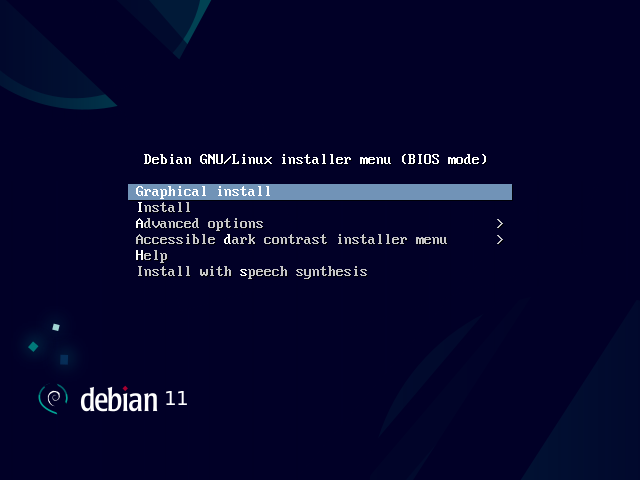
\includegraphics{img001.png}
	\caption{\label{fig-first-screen}Le premier écran de l'installateur.}
\end{figure}

Une fois le fichier ISO gravé sur le support et l'ordinateur démarré sur ce même support un premier écran s'affichera, celui de la capture précédente.

Comme vous le voyez, les images étant grandes et ne voulant pas surcharger inutilement tant la connexion internet si, comme je le 
présume, la page est consultée depuis un téléphone ou via une connexion limitée, j'ai décidé de retailler toutes les images qui suivront. 
Aussi toutes les captures qui suivent contiendront les éléments nécessaires à la compréhension des choix à effectuer pour une installation de nature similaire à celle que j'ai produite.

Je n'aime pas utiliser l'installation basique qu'elle soit textuelle (Install) ou qu'elle soit graphique (Graphical install) aussi je passe toujours par l'option (Advanced options).

\begin{figure}
	\centering
	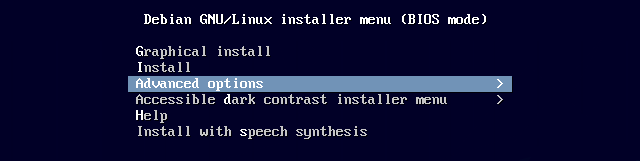
\includegraphics{img002.png}
	\caption{Sélection des options avancées.}
\end{figure}

Une fois l'option avancée choisie, pour les besoins de cette installation j'ai opté exceptionnellement pour pour l'installation en mode expert et graphique. 
Un accident totalement involontaire a cependant fait échouer avant la fin l'installation et, par habitude, la seconde installation identique, s'est faite en mode textuel, aussi les dernières captures d'écran seront différentes de celles du début.

Après quelques secondes une fois le choix effectué l'écran de la capture suivant apparaît.

\begin{figure}
	\centering
	
\includegraphics{img003.png}
	\caption{Le sous-menu d'options avancées.}
\end{figure}

Cette capture nous montre la voie à suivre et les différentes étapes qui seront parcourrues pendant l'installation. 
Pour choisir un des items dans l'une des différentes étapes il suffit de se déplacer avec les flèches directionnelles du clavier ou avec la souris lors d'une installation graphique et pour choisir il suffit de valider par la touche entrée ou de cliquer sur le bouton \fbox{{\tt continuer}} qui apparaît en bas à droite dans la plupart des captures d'écran.

La première partie sera évidemment de choisir la langue utilisée lors de l'installation. La langue anglaise est peut-être votre tasse de thé mais pas la mienne aussi ...

\chapter{La langue et les localisations}

Mais commençons par le commencement. 
\emph{Debian} gère de nombreuses langues officielles et régionales, aussi afin de pouvoir communiquer avec nous, le programme d'installation nous demande d'effectuer une sélection linguistique.

\begin{figure}
	\centering
	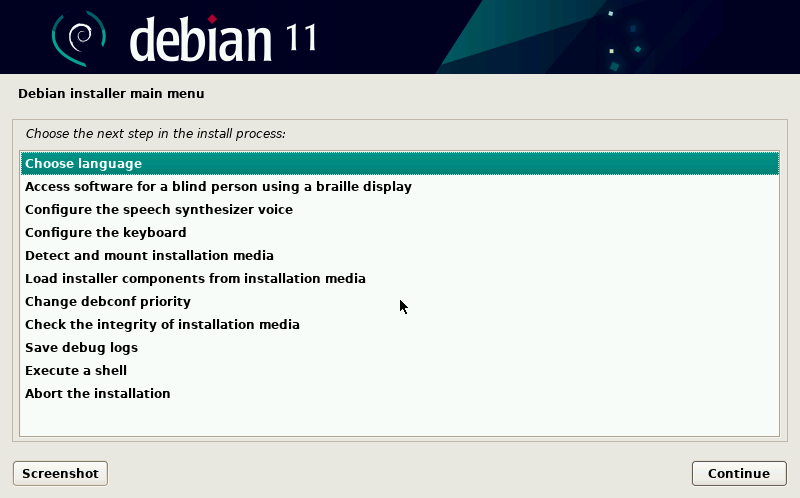
\includegraphics{img004.png}
	\caption{Menu principal : choix de la langue.}
\end{figure}

Même si j'aime bien la langue ce \emph{Shakespeare} et que je suis un inconditionnel \emph{amante} de celle de \emph{Cervantes} ... je préfère basculer vers la langue française et ainsi me faire plaisir, \emph{Molière} ou \emph{Racine} et tous les autres auteurs du passé ne m'en voudront pas de ne pas les citer tous et toutes.

\begin{figure}
	\centering
	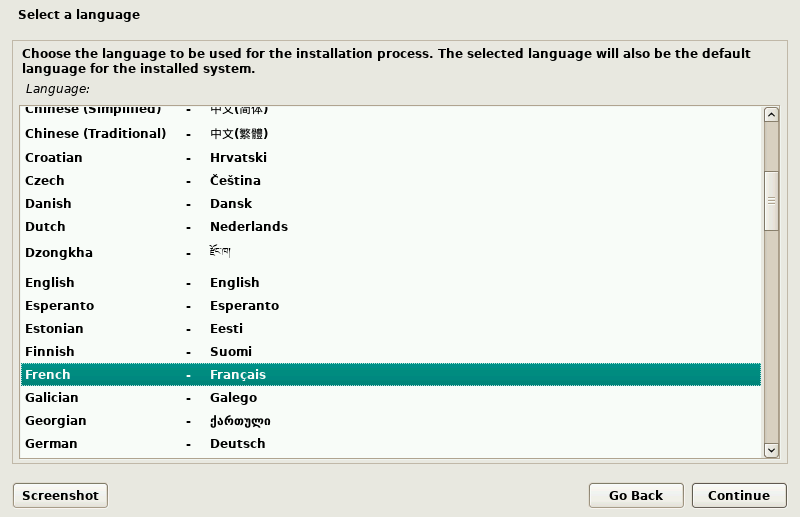
\includegraphics{img005.png}
	\caption{Le Français !!!}
\end{figure}

La langue d'installation étant fixée, la suite consiste à choisir la localisation géographique, parmi les différents pays de langue francophone, je choisis évidemment la France ...

\begin{figure}
	\centering
	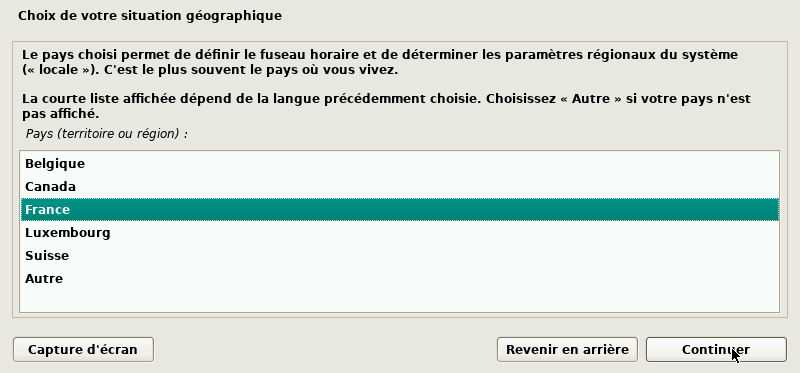
\includegraphics{img006.png}
	\caption{La France qu'on vous dit !}
\end{figure}

... il faut bien sûr fixer ensuite les locales, c'est-à-dire les paramètres régionaux du système futur.

\begin{figure}
	\centering
	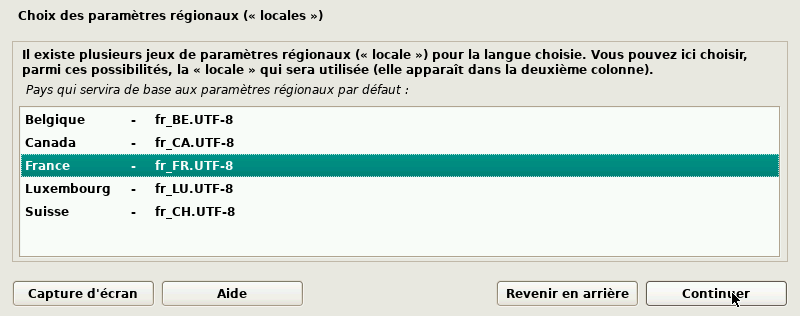
\includegraphics{img007.png}
	\caption{Choix de la locale du futur système.}
\end{figure}

Le système Linux admet plusieurs paramètres régionaux ce qui peut avoir son utilité dans certaines situations, ici le système qui est sur le point d'être installé n'aura pas besoin de ces ajouts aussi aucune case n'est cochée dans la capture suivante.

\begin{figure}
	\centering
	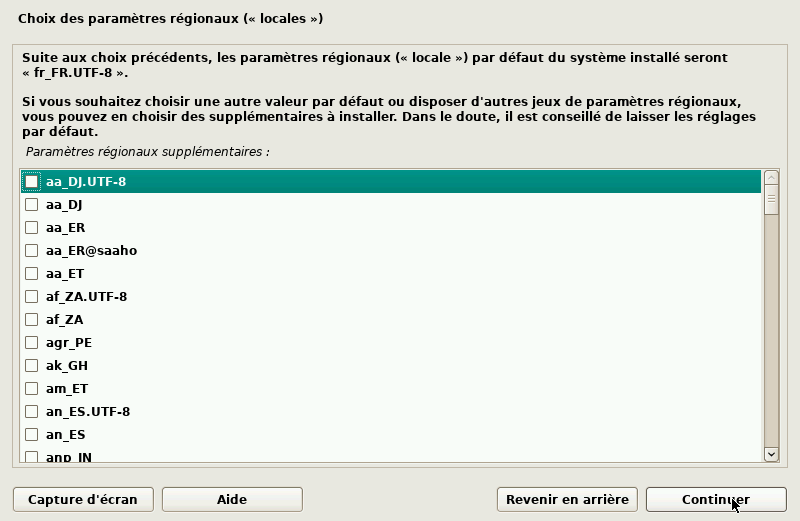
\includegraphics{img008.png}
	\caption{D'autres locales disponibles.}
\end{figure}

Arrivé(e) à ce stade la langue, le pays et la langue de l'interface est déterminée et fixée pour le reste de l'installation tout comme pour le futur système opératif.

\chapter{Les adaptations aux personnes handicapées}

Le système GNU/Linux \emph{Debian} se voulant le plus ouvert et large, le support des dispositifs braille est inclus dès cette étape. 
Si aucun dispositif de la sorte n'est détecté -- ce qui est le cas dans mes configurations -- alors l'appui sur continuer ou sur entrée ne fait que passer à l'étape suivante ...

\begin{figure}
	\centering
	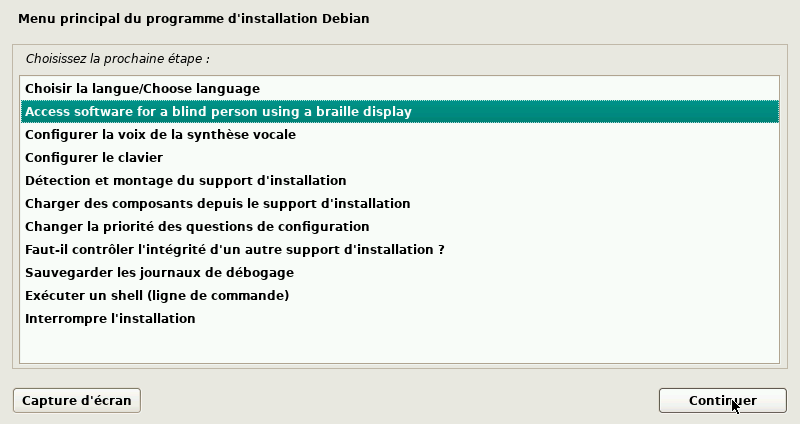
\includegraphics{img009.png}
	\caption{Vérification de la présence d'un terminal braille.}
\end{figure}

... celle de la configuration de la synthèse vocale. 
Également absent de mes ordinateurs, la validation ou la continuation aura un effet similaire à savoir le passage à l'étape ultérieure.

\begin{figure}
	\centering
	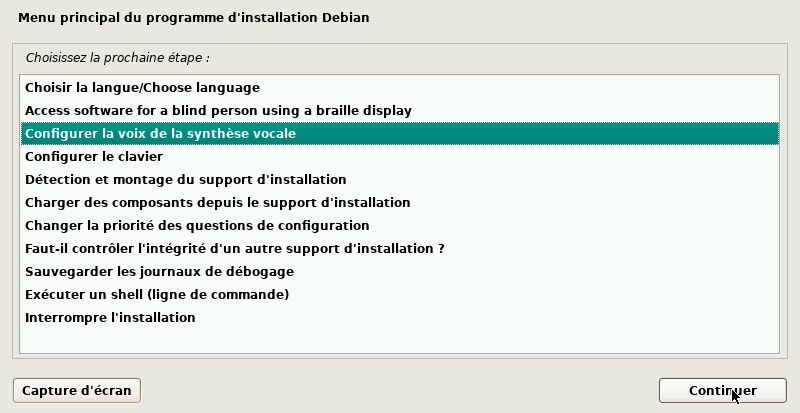
\includegraphics{img010.png}
	\caption{Mise en place d'une synthèse vocale... peut-être.}
\end{figure}

Je pense que comme aucun dispositif de la sorte n'est présent sur mon système, aucune assistance vocale à l'installation n'est alors proposée dans la seconde captures, c'est pour cela que le clic sur le bouton \fbox{{\tt Continuer}} ne provoque rien d'autre que le passage à l'étape ultérieure.

\chapter{La configuration du clavier}

Une fois tous ces paramètres fixés restent les paramètres du clavier. 

\begin{figure}
	\centering
	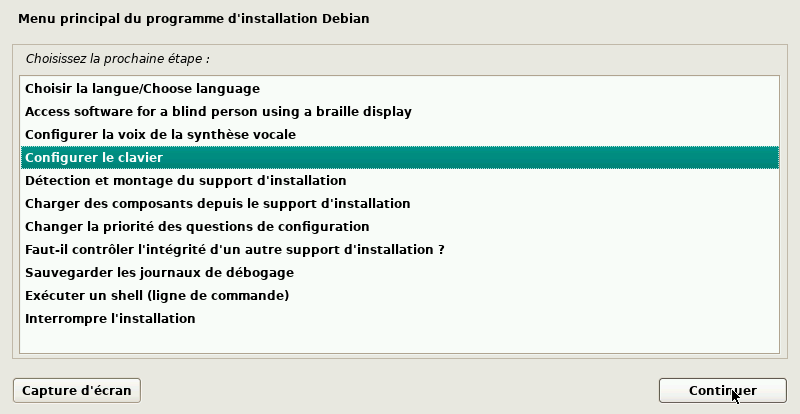
\includegraphics{img011.png}
	\caption{Menu principal : Configuration du clavier.}
\end{figure}

Clavier qui est automatiquement sélectionné en Français vu les locales paramétrées précédemment.

\begin{figure}
	\centering
	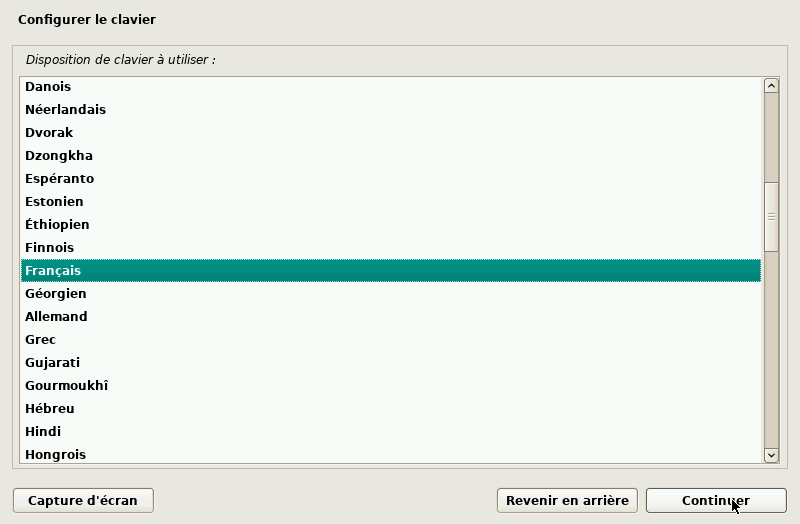
\includegraphics{img012.png}
	\caption{Choix de la langue du clavier pour l'installation et pour le système cible.}
\end{figure}

\chapter{Vérification du support.}

Avant de poursuivre, l'installateur se doit de vérifier l'intégrité du contenu du support. 
Un seul paquet impropre et tôt ou tard lors de l'installation, une erreur critique se manifestera et gèlera aussitôt la mise en place du système.

\begin{figure}
	\centering
	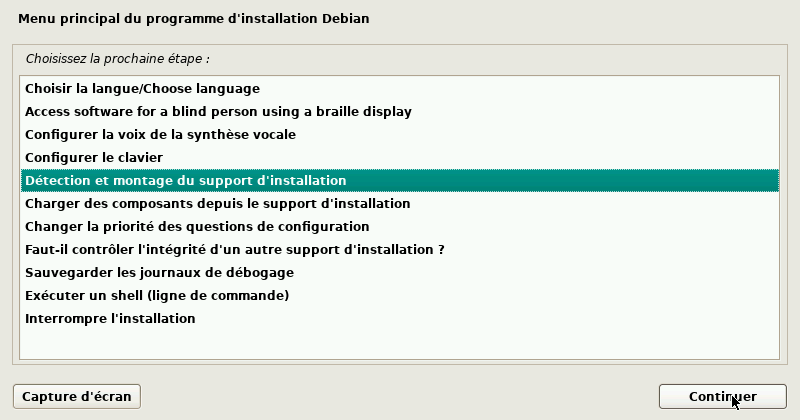
\includegraphics{img013.png}
	\caption{Menu principal : Détection et montage du support d'installation.}
\end{figure}

Les modules obligatoires pour poursuivre sont automatiquement cochés. 

\begin{figure}
	\centering
	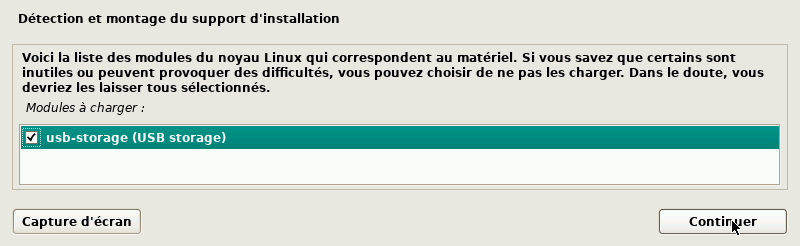
\includegraphics{img014.png}
	\caption{Chargement automatique du support de l'USB pour la suite de l'installation.}
\end{figure}

Si tout va bien, ce magnifique message apparaîtra.

\begin{figure}
	\centering
	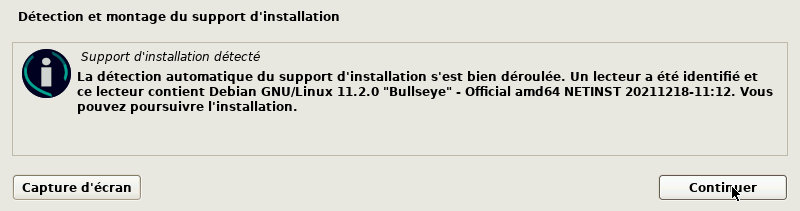
\includegraphics{img015.png}
	\caption{Le support est reconnu, accepté et intègre.}
\end{figure}

Tout est donc prêt pour continuer.

\chapter{Chargement d'outils supplémentaires.}

\begin{figure}
	\centering
	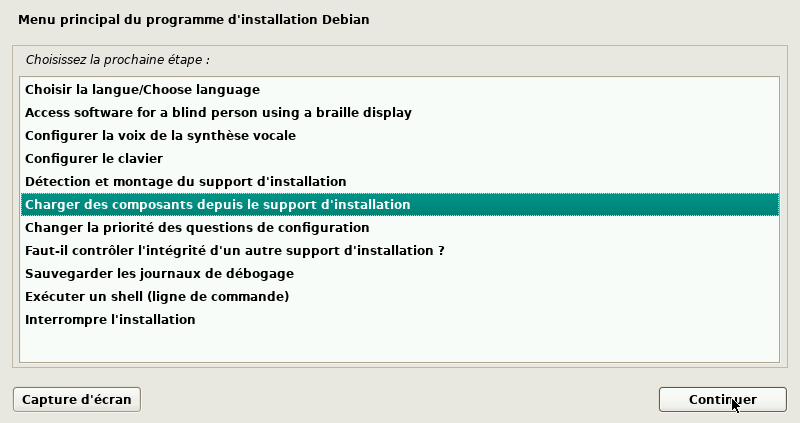
\includegraphics{img016.png}
	\caption{Menu principal : Charger les composants depuis le support.}
\end{figure}

Comme le montre la capture précédente la ligne suivante sera sélectionnée pour charger les composants supplémentaires. 
Le message indique que lors d'une détection interne si des modules s'avèrent nécessaires ils seront automatiquement chargés. 
La liste proposée ne contient que les composants que le système ne détecte pas mais que l'utilisateur sait être importants pour sa personnalisation.

\begin{figure}
	\centering
	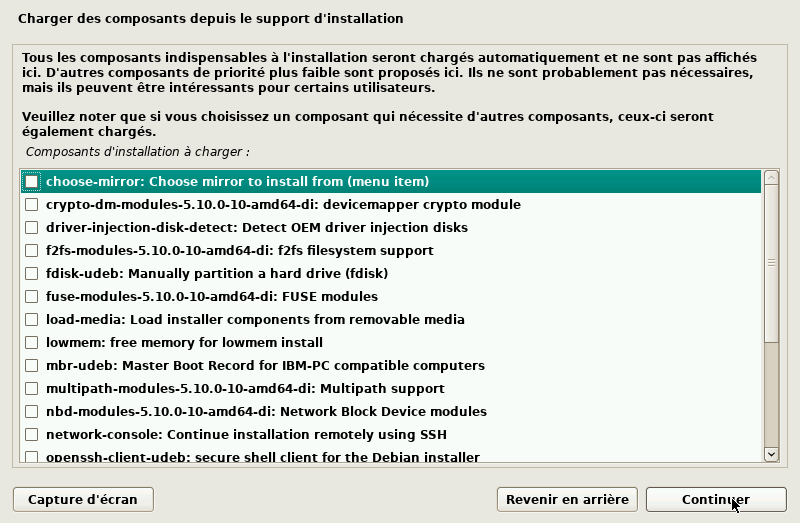
\includegraphics{img017.png}
	\caption{Choix de composants supplémentaires non détectés à ce stade par l'installateur.}
\end{figure}

Avant de poursuivre il peut être nécessaire d'insérer des modules autres que le système n'estime pas obligatoire. Par exemple si on décide qu'on va utiliser un miroir d'installation local (donc non proposé : {\tt choose-mirror}), ou bien si un des disques est chiffré et qu'on souhaite le conserver ({\tt crypto-dm-modules}), ou encore si la machine a très peu de mémoire vive (lowmem) voir si on souhaite installer le minimum du minimum pour finir l'installation dans une seconde étape à distance ({\tt network-console}) ...

Après avoir coché ou non certaines cases et aussi coché le bouton \fbox{{\tt Continuer}} le chargement automatique des modules cochés 

\begin{figure}
	\centering
	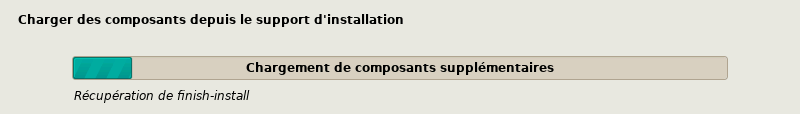
\includegraphics{img018.png}
	\caption{Progression du chargement des composants supplémentaires.}
\end{figure}

Bien ! 
Nous sommes prêts, modules et pilotes chargés, à attaquer la suite des opérations avec la configuration du réseau.

\chapter{La partie réseau.}

Ici arrive la configuration cruciale pour la suite même si elle ne représente pas la partie la plus importante de cette production.

\begin{figure}
	\centering
	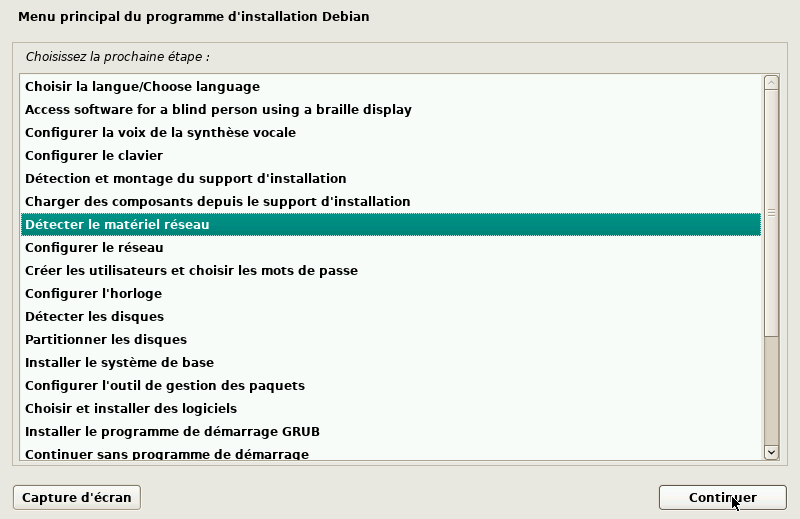
\includegraphics{img019.png}
	\caption{Menu principal : détection du matériel réseau.}
\end{figure}

Cette étape commence par la détection du matériel réseau. 
Si cette dernière est reconnue alors s'affichera la capture suivante pour la configuration.

\begin{figure}
	\centering
	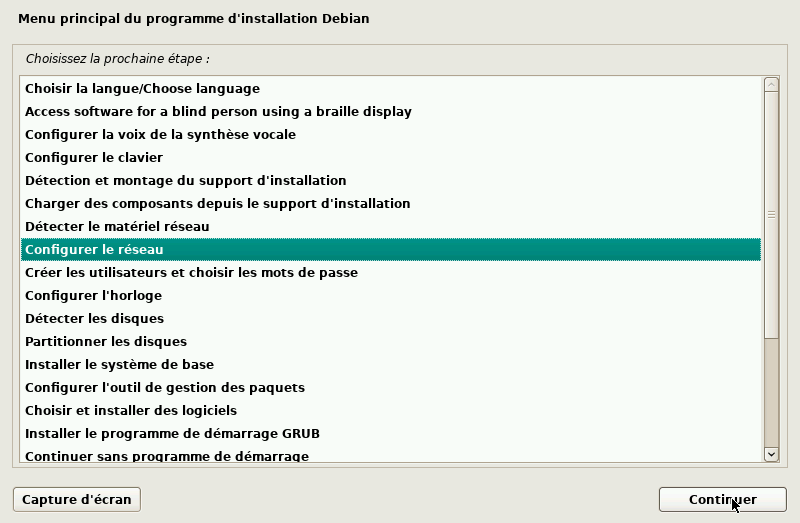
\includegraphics{img020.png}
	\caption{Menu principal : configuration du réseau.}
\end{figure}

Si plusieurs cartes sont disponibles, une page intermédiaire va demander de choisir laquelle sera utilisée. Les cartes réseaux peuvent s'appeler de différentes façons :
\begin{itemize}
	\item les cartes réseau filaires (ethernet) : les anciens noms sont {\tt eth0}, {\tt eth1}, etc... les nouveaux noms sont {\tt enpXsY} où X et Y sont des chiffres dépendant des cartes, ou enoX, ou d'autres noms encore plus étranges.
	\item les cartes réseau sans-fil (wi-fi) : les anciens noms sont {\tt wlan0}, {\tt wlan1}, etc... les nouvelles s'appellent aussi {\tt wlpXsY} où X et Y peuvent changer en fonction de la carte réseau et de l'ordinateur
\end{itemize}

Au final, lorsque la carte est choisie l'écran suivant va apparaître proposant la configuration automatique du réseau. Dans le cas où il n'y a pas besoin de jouer avec les paramètres, autant laisser le choix `` oui''.

\begin{figure}
	\centering
	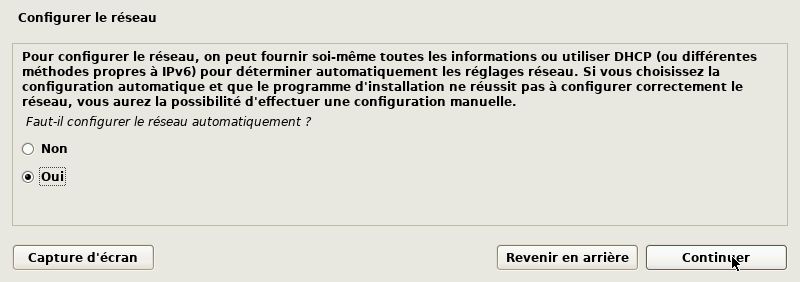
\includegraphics{img021.png}
	\caption{Proposition de configuration automatique de la carte sélectionnée.}
\end{figure}

\paragraph{Attention :} si le choix est "non" alors il faudra savoir quelques éléments de configuration réseau à savoir :
\begin{itemize}
	\item l'adresse du sous-réseau ethernet (souvent commençant par 192.168) 
	\item l'adresse dans ce sous-réseau qu'on souhaite attribuer à la machine 
	\item la passerelle de ce sous-réseau pour sortir vers Internet
	\item le masque de ce sous-réseau pour communiquer par défaut seulement au sein de ce sous-réseau (souvent 255.255.255.0)
	\item l'adresse {\tt IP} du serveur de résolution des noms de domaines (DNS) qui souvent correspond à celui de la passerelle dans une connexion domestique.
\end{itemize}

\begin{figure}
	\centering
	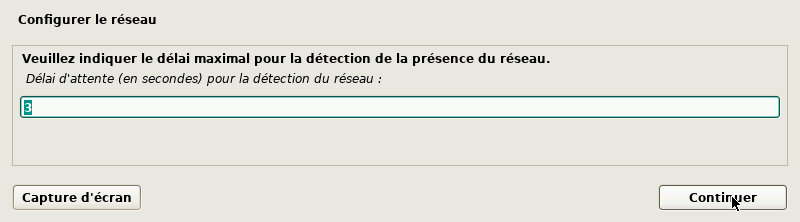
\includegraphics{img022.png}
	\caption{Indication du temps d'attente avant la détection du réseau.}
\end{figure}

Ensuite autant laisser les 3 secondes nécessaires au démarrage de la carte afin qu'elle soit parfaitement alimentée avant de détecter les connexions réseaux.

\begin{figure}
	\centering
	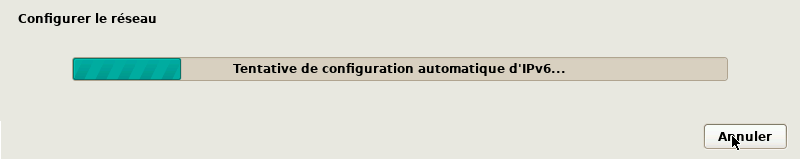
\includegraphics{img023.png}
	\caption{Configuration de l'{\tt IP} version 6.}
\end{figure}

D'abord l'{\tt IP} version 6 sera configurée automatiquement puis se sera le tour de l'{\tt IP} version 4 d'être configurée automatiquement.

\begin{figure}
	\centering
	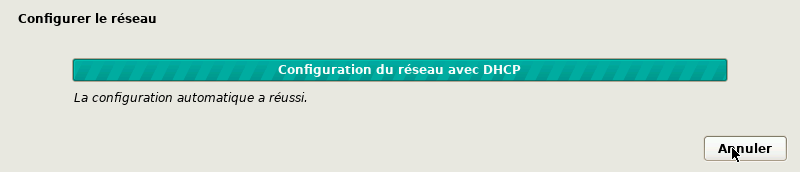
\includegraphics{img024.png}
	\caption{Configuration de l'{\tt IP} version 4.}
\end{figure}

Le point suivant correspond à la configuration du nom de la machine cela semble futile pourtant tous les systèmes, même \emph{Windows} nécessite un nommage de chaque machine afin de leur permettre une communication en réseau local, par défaut \emph{Debian} est proposé mais chacun et chacune peut proposer de qu'il veut dans la limite des caractères acceptés.

\begin{figure}
	\centering
	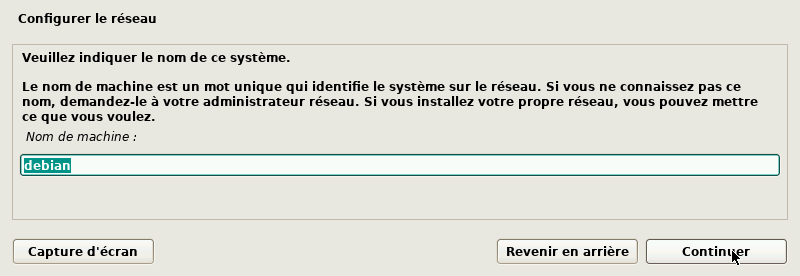
\includegraphics{img025.png}
	\caption{Choix du nom de la machine.}
\end{figure}

Pour parachever la configuration réseau il est important de préciser si c'est le cas, le nom du domaine dans lequel la machine est ou sera présente, si vous laissez vide aucun soucis (au pire cela se paramètre ultérieurement) puisque chez soi aucun nom particulier n'est donné au réseau (sauf situations exceptionnelles).

\begin{figure}
	\centering
	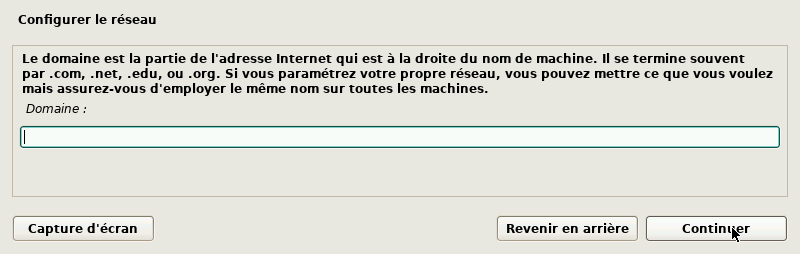
\includegraphics{img026.png}
	\caption{Choix du nom du domaine où réside la machine.}
\end{figure}

La configuration est finie, il est l'heure de passer à celle du ou des utilisateurs futurs de cette machine.

\chapter{Le ou les utilisateurs}

Lorsqu'on installe un système \emph{Debian} par défaut ce qui est le cas dans celle détaillée au sein de ce document, il y a création de deux utilisateurs différents : {\tt root} l'administrateur et un autre pour les usages basiques. 
La création de {\tt root} est alors automatisée et ne peut être refusée.

\begin{figure}
	\centering
	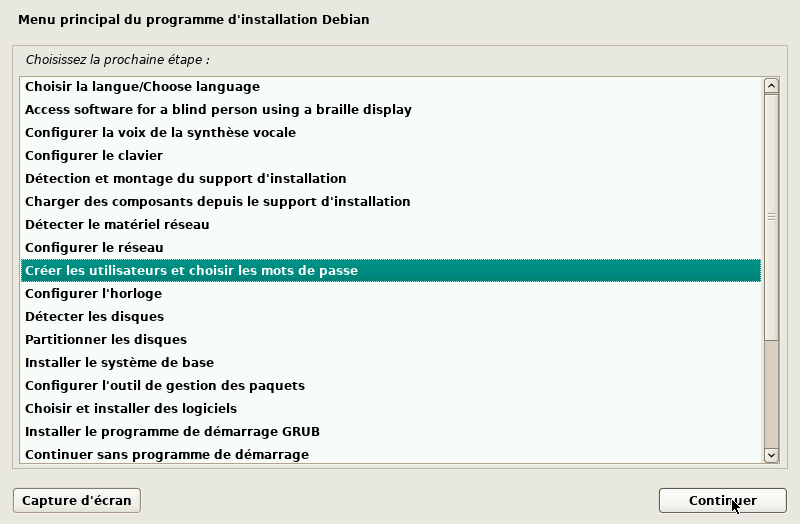
\includegraphics{img027.png}
	\caption{Choix de création d'utilisateurs.}
\end{figure}

En passant par les options avancées il nous est proposé de ne pas créer de {\tt root}, \emph{de facto} l'utilisateur standard créé se voyait affublé de droits supplémentaires en faisant partie du groupe {\tt sudo} lui octroyant pour une grande partie les mêmes possibilités que l'administrateur {\tt root}.

\begin{figure}
	\centering
	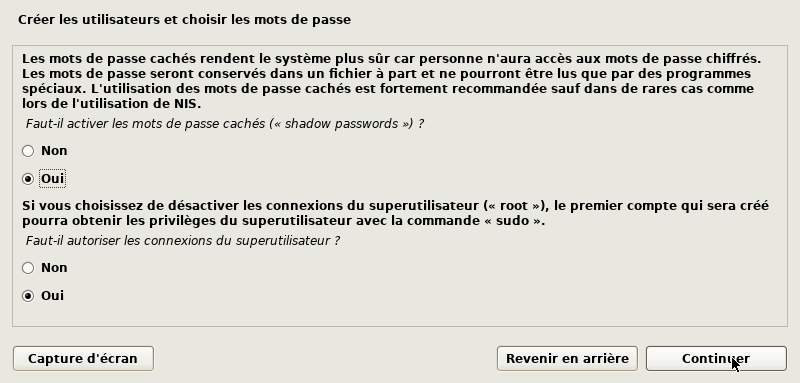
\includegraphics{img028.png}
	\caption{Protection des mots de passe et autorisation du login de {\tt root}.}
\end{figure}

À cette étape sera demandé s'il faut protéger les mots de passe en utilisant le fichier {\tt /etc/shadow}\footnote{shadow : Aux premiers temps du système UNIX et donc par essence, Linux le fichier {\tt /etc/passwd} contenait les mots de passes des utilisateurs en clair. Évidemment cela posait de sérieux problèmes en cas d'accès au système. Dans l'optique d'une sécurité accrue, il fût mis en place le fichier {\tt /etc/shadow} qui contient un \emph{hash} du mot de passe, non plus le mot de passe lui-même, permettant ainsi de sécuriser plus cette authentification.} et s'il faut autoriser ou pas la connexion du compte {\tt root}.

Si le compte {\tt root} est autorisé, la création du compte utilisateur à une étape ultérieure n'inscrira pas cet utilisateur dans le groupe des administrateurs ({\tt sudo}) par contre si le compte {\tt root} n'est pas autorisé à se connecter alors l'utilisateur sera dans {\tt sudo}.

\begin{figure}
	\centering
	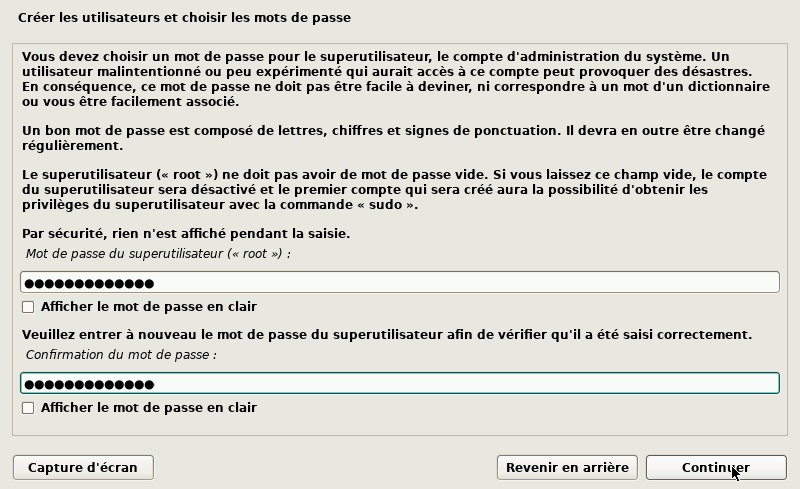
\includegraphics{img029.png}
	\caption{Mot de passe de root.}
\end{figure}

Suite à quoi sera créé le compte {\tt root} et le mot de passe sera demandé deux fois (notez qu'on peut le faire apparaître pour le vérifier à cet instant précis ça ne sera plus le cas ultérieurement.

Vous aurez noté la présence d'une case à cocher pour afficher le mot de passe en clair ce qui est important à cet instant de l'installation surtout quand on ne connaît pas finement la gestion du clavier dans Linux.

\begin{figure}
	\centering
	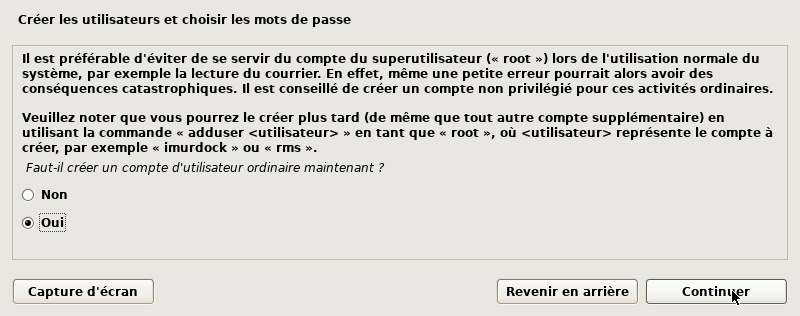
\includegraphics{img030.png}
	\caption{Création de l'utilisateur standard.}
\end{figure}

À cette étape est demandé si un utilisateur standard est nécessaire, cette question apparaît lorsque le compte {\tt root} a été précédemment été autorisé à se connecter car si ça n'avait pas été le cas, la création du compte utilisateur est obligatoire.

\begin{figure}
	\centering
	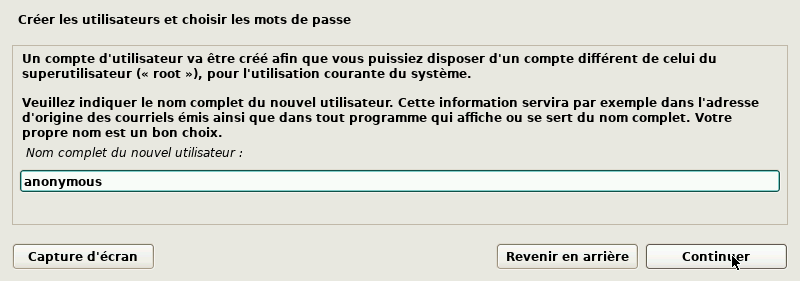
\includegraphics{img031.png}
	\caption{Création du nom complet.}
\end{figure}

Suite à cette question, il faut évidemment rentrer le nom complet de l'utilisateur (nom, prénom, ce que vous voulez) ...

\begin{figure}
	\centering
	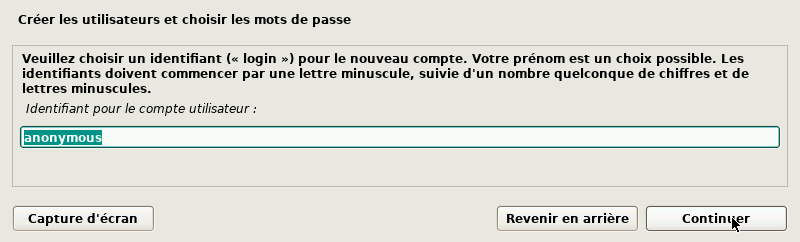
\includegraphics{img032.png}
	\caption{Création du \emph{username}}
\end{figure}

... puis le nom d'utilisateur au sens {\tt UNIX} du terme (pas d'accents, pas d'espaces, etc.), ce nom d'utilisateur s'utilisera principalement dans les terminaux en mode textuel pur ou en mode graphique.

\begin{figure}
	\centering
	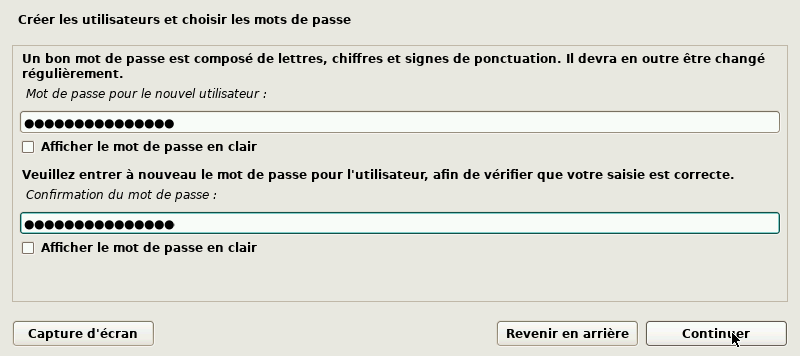
\includegraphics{img033.png}
	\caption{[Mot de passe de l'utilisateur.}
\end{figure}

Tout comme pour {\tt root}, le mot de passe est masqué mais peut être rendu visible par l'activation de la casse idoine.

Le ou les comptes d'utilisateurs du futur système sont donc prêts à être installés le moment venu, il va falloir passer à l'étape suivante de configuration de l'horloge système ce qui revêt une certaine importance traitée au chapitre suivant.

\chapter{Réglage de l'horloge et du fuseau horaire.}

Cette partie va s'avérer importante dans certains cas, pas tant pour l'utilisateur d'un poste de travail classique -- quoi que cela puisse avoir son importance -- mais il ne faut pas oublier que \emph{Debian} reste dans sa conception et son ADN une distribution orientée serveurs.

Or, afin que tous les serveurs partout dans le monde soient réglés comme il faut les machines fonctionnant sous Linux seul ont comme habitude de régler l'horloge matérielle de l'ordinateur sur le temps universel GMT et d'appliquer un décalage dû au fuseau horaire.

\begin{figure}
	\centering
	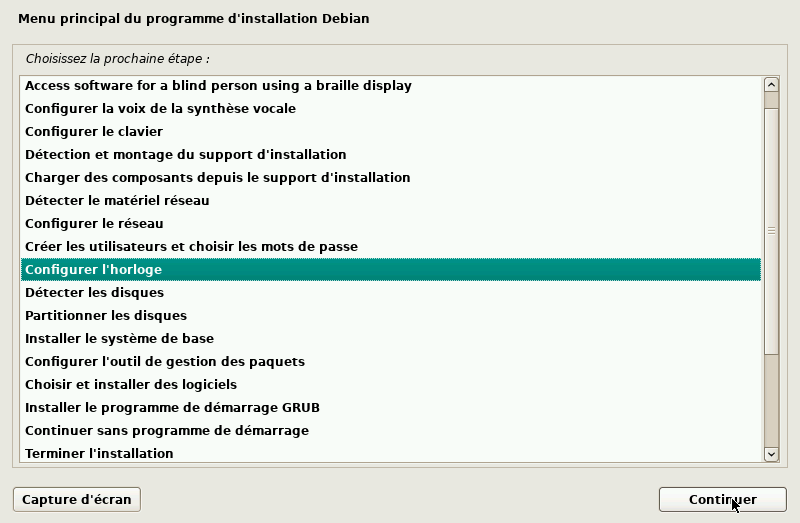
\includegraphics{img034.png}
	\caption{Menu principal : configuration de l'horloge.}
\end{figure}

Une machine fonctionnant sous \emph{Windows} voit son heure matérielle dans le même fuseau horaire que celle du système, pas sous Linux et sous {\tt macOS} également.

D'ailleurs -- j'écris cela de mémoire -- Microsoft (\emph{Windows}) utilise lui aussi un service de temps pour la même chose mais il est rarement actif par défaut.

Afin d'assurer le bon réglage des heures les unes par rapport aux autres il est demandé s'il faut utiliser le service NTP\footnote{N.T.P. : Network Time Protocole, c'est une protocole de communication vers des sites offrant une heure synchronisée afin que tous les serveurs soient synchronisés partout sur la Terre.} pour synchroniser l'horloge du système.

\begin{figure}
	\centering
	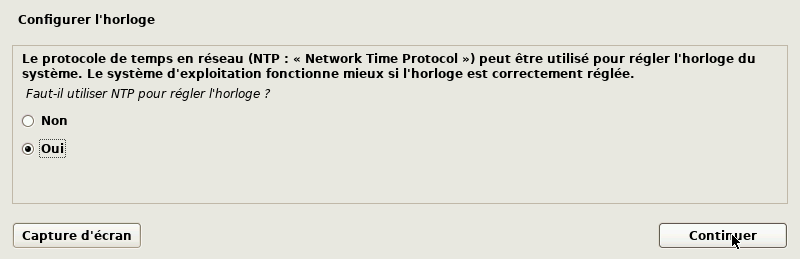
\includegraphics{img035.png}
	\caption{Demande d'activation du service NTP}
\end{figure}

Par défaut le choix étant "oui" la fenêtre suivante est proposée, elle utilise le serveur faisant tourner le service (côté serveur) pour effectuer les recalages.

Sauf si vous connaissez l'adresse exacte d'un serveur de temps, ne pas toucher à ce paramètre est judicieux.

\begin{figure}
	\centering
	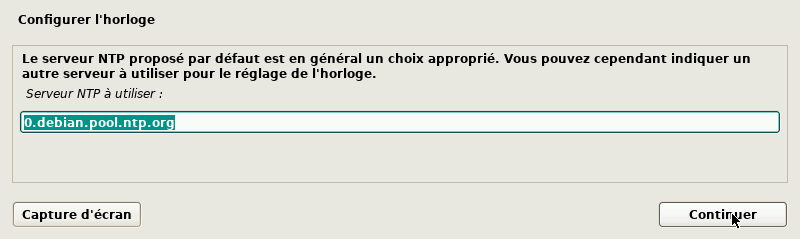
\includegraphics{img036.png}
	\caption{Configuration de l'adresse du serveur offrant le service NTP}
\end{figure}

Si la connexion s'établit vers le dit serveur, le fuseau horaire le plus proche entre vos réglages linguistiques, l'heure système et l'horloge matérielle sera proposé en plus du temps universel.

\begin{figure}
	\centering
	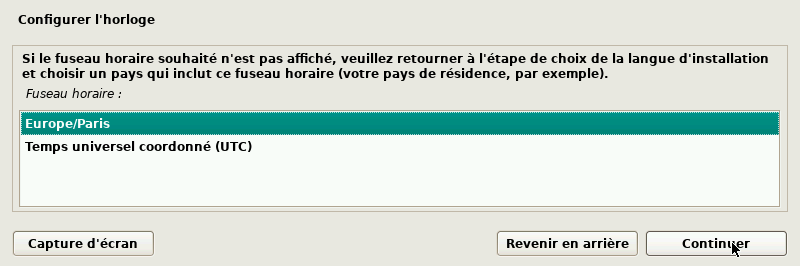
\includegraphics{img037.png}
	\caption{Sélection du fuseau horaire.}
\end{figure}

Ces réglages sont importants surtout pour la validité des certificats et des signatures cryptographiques utilisées par certains services et ou logiciels. 
Au moment de la fin de validité d'un tel document ou au début de la validité d'un autre, si l'horloge est mal réglée c'est

\chapter{Préparation du support}

\begin{figure}
	\centering
	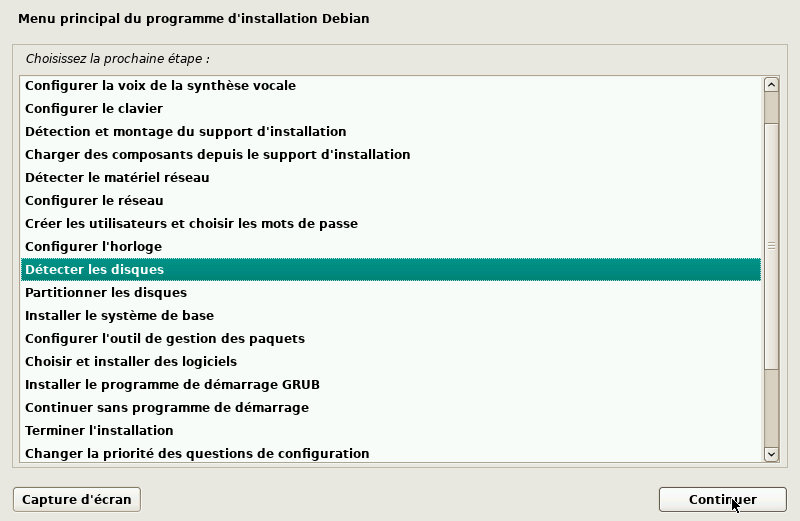
\includegraphics{img038.png}
	\caption{Menu principal : Détection des disques.}
\end{figure}

On va désormais se concentrer sur le support de la future installation \emph{i.e.} le disque dur interne.

Dans ce document j'ai opté pour une installation chiffrée sauf le dossier {\tt boot} qui sera quant à lui laissé à l'extérieur du chiffrement. 
C'est un choix délibéré de ma part car l'installateur basique ne permet pas mieux comme possibilité nativement, c'est-à-dire sans sortir de lui-même par l'exécution d'un script {\tt bash}.

Dans les méthodes de chiffrement il existe pléthore de possibilités mais je préfère malgré tout l'utilisation d'une configuration relativement simple :
\begin{itemize}
	\item un dossier {\tt /boot} en clair pour le démarrage
	\item le reste du disque chiffré via {\tt luks}.
	\begin{itemize}
		\item dans le volume chiffré {\tt luks} un \emph{logical volume manager} (\emph{LVM})
		\begin{itemize}
			\item dans ce {\tt lvm} un groupe qui contiendra le système
			\begin{itemize}
				\item dans ce groupe {\tt /swap} et {\tt /home}
			\end{itemize}
		\end{itemize}
	\end{itemize}
	\item pas d'{\tt EFI} évidemment
\end{itemize}

Concernant les variantes pour une machine avec {\tt EFI} il y a un chapitre spécifique en annexe.

La première étape consiste donc à détecter le ou les disques présents au sein du système puisque Linux sait parfaitement gérer un système dispersé sur plusieurs disques.

S'exécute alors l'outil de partitionnement ...

\begin{figure}
	\centering
	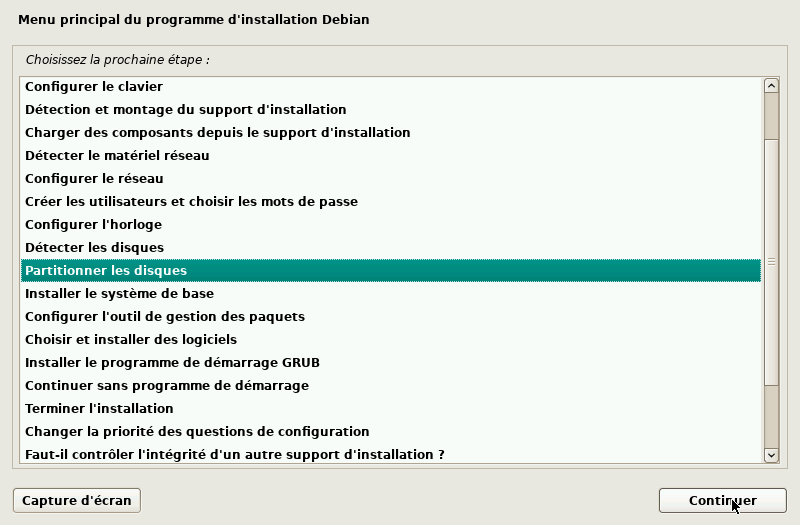
\includegraphics{img039.png}
	\caption{Menu principal : Partitionnement des disques.}
\end{figure}

... ce qui va nécessiter le chargement des composants utiles pour la gestion du chiffrement et des volumes logiciels...

\begin{figure}
	\centering
	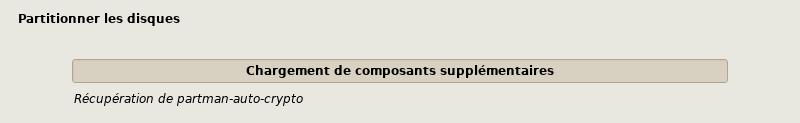
\includegraphics{img040.png}
	\caption{Barre de progression de chargement des outils supplémentaires.}
\end{figure}

... et le chargement de de l'outil graphique ou semi-graphique de partitionnement.

\begin{figure}
	\centering
	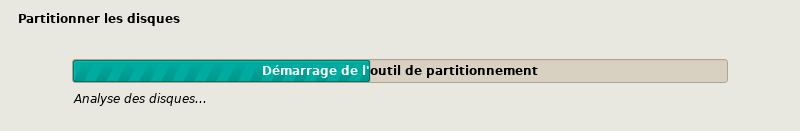
\includegraphics{img041.png}
	\caption{Barre de progression du chargement des outils de partitionnement.}
\end{figure}

Plusieurs choix sont offerts~:
\begin{itemize}
	\item si vous n'y connaissez rien ou avez peu confiance en vos capacités, le premier choix "Assisté - utiliser un disque entier" est l'option la plus sûre et aussi la moins fine mai au moins vous aurez l'impression de facilité à l'installatino de la distribution \emph{Debian}.
	\item le choix "Assisté - utiliser tout un disque avec LVM" et une option qui se rapproche de ce que je veux mettre en place, mais il manque le chiffrement protecteur que désire mettre en place.
	\item Ensuite le choix "Assisté - utiliser un disque avec LVM chiffré" est le choix qui se rapproche le plus de que je souhaite mettre en place. Il manque cependant une finesse dans le partitionnement comme la séparation des partitions utilisateur et racine ainsi qu'un meilleur contrôle du \emph{swap}.
\end{itemize}

Aussi mon choix se portera concrètement sur {\tt Manuel} me laissant plus grande autonomie et liberté dans la configuration.

\begin{figure}
	\centering
	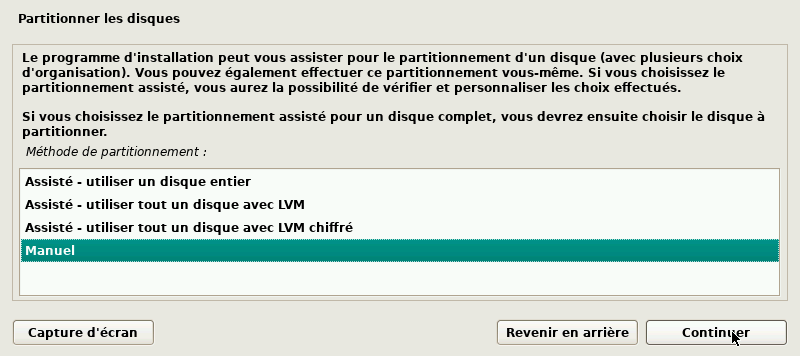
\includegraphics{img042.png}
	\caption{Partitionnement : création d'une table de partitionnement.}
\end{figure}

Dans l'image sur la création d'une table de partitionnement comme le disque est totalement neuf et non partitionné en usine, il n'y a aucune table déterminée.

Lorsque je crée une table de partition nouvelle sur un disque deux choix s'offrent à moi sur un disque fonctionnant dans un ordinateur de type {\tt PC}, soit un partitionnement {\tt MS-DOS} ou {\tt DOS} soit un partitionnement {\tt GPT}.

\begin{figure}
	\centering
	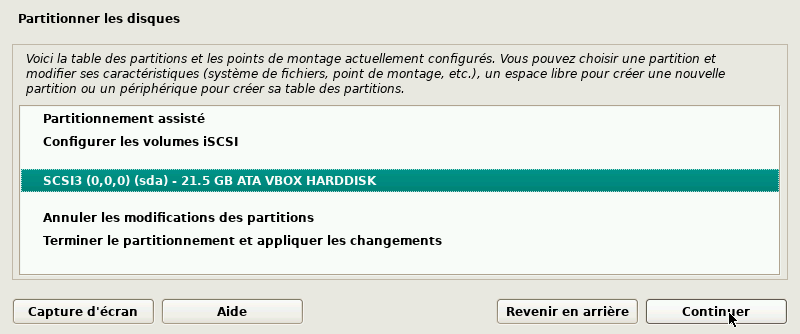
\includegraphics{img043.png}
	\caption{Sélection du disque {\tt VBOX HARDDISK} pour l'installation.}
\end{figure}

Étant donné que l'installation se fait ici sur une machine virtuelle simulant un ordinateur de type {\tt PC} avec {\tt BIOS} (et non {\tt EFI}) la table de partition sera de type {\tt msdos}.

Cela signifie que je pourrai définir jusqu'à 4 partitions primaires et en cas de nécessité de plus, une partition primaire peut être utilisée pour créer jusqu'à une vingtaine de partitions secondaires.

Le cas d'un système avec {\tt EFI} sera traité dans un document spécifique.

\begin{figure}
	\centering
	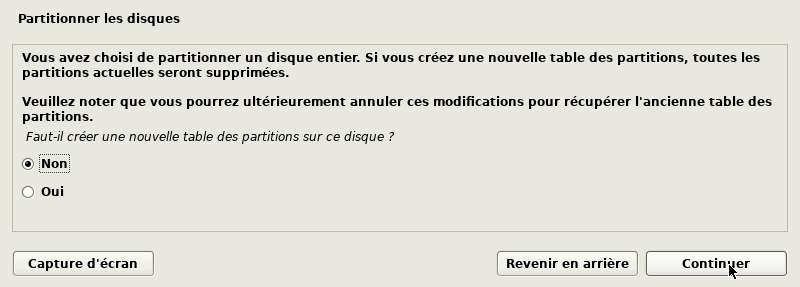
\includegraphics{img044.png}
	\caption{Faut-il créer une table de partition ? Bien sûr !}
\end{figure}

Évidemment le système demande si une nouvelle table de partition doit être créée dans ce disque qui n'en possède aucune -- ce qui n'est pas le cas pour les disques du commerce qui en ont déjà une.

%<!-- ![45](img045.png} doublon inutile -->

\begin{figure}
	\centering
	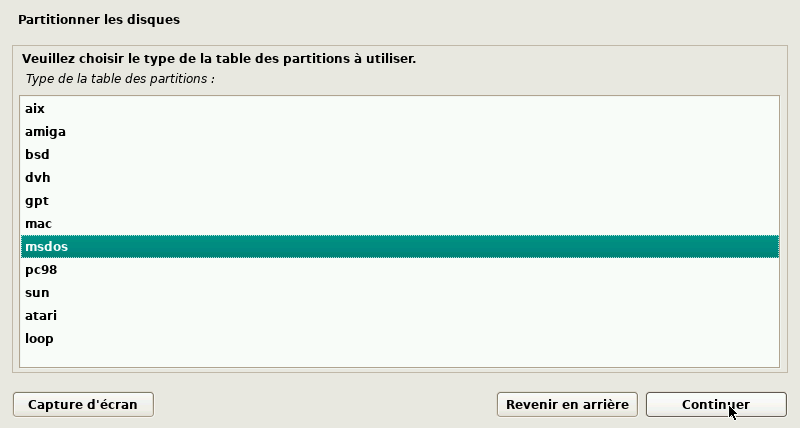
\includegraphics{img046.png}
	\caption{Choix de la table de partition {\tt MS-DOS}.}
\end{figure}

Évidemment ce sera une table de type {\tt MS-DOS} avec les restrictions idoine à ce type de table de partitionnement.

Le résultat se voit à l'écran suivant : un espace libre apparaît désormais dans la ligne placée sous celle désignant le disque, il va falloir désormais créer les partitions.

\begin{figure}
	\centering
	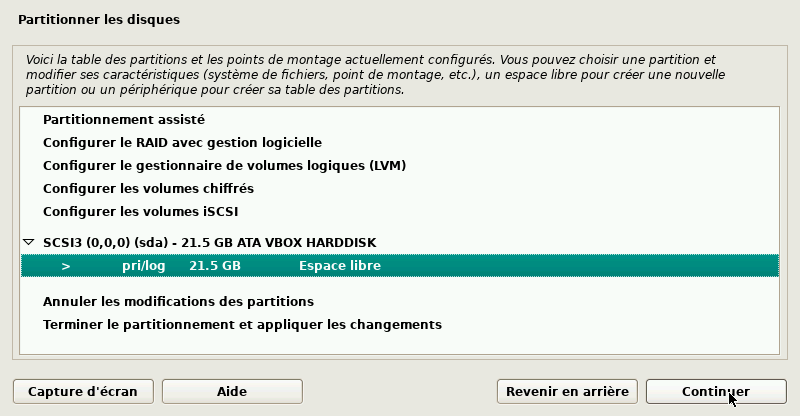
\includegraphics{img047.png}
	\caption{Enfin de l'espace libre.}
\end{figure}

En double cliquant sur l'espace libre -- ou en validant avec la touche entrée -- on arrive alors à cette nouvelle fenêtre qui nous propose trois choix -- d'autres options seraient possibles si des partitions préexistaient.

\begin{figure}
	\centering
	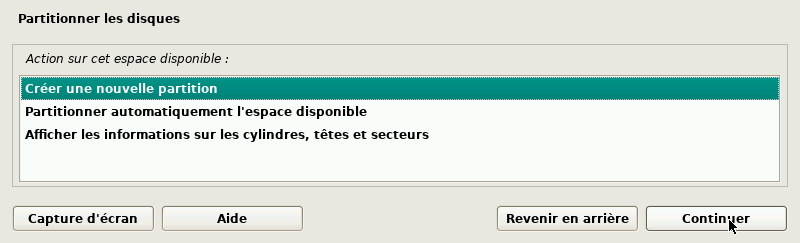
\includegraphics{img048.png}
	\caption{Créer une nouvelle partition, simple non ?}
\end{figure}

Il m'est bien sûr demandé la taille de cette partition, je peux saisir ce que je veux en respectant quelques règles élémentaires :
\begin{itemize}
	\item le séparateur décimal est le point, à l'anglosaxone,
	\item indiquer la valeur en GB (Gigaoctets/GibaBytes), MB, kB ...
\end{itemize}

\begin{figure}
	\centering
	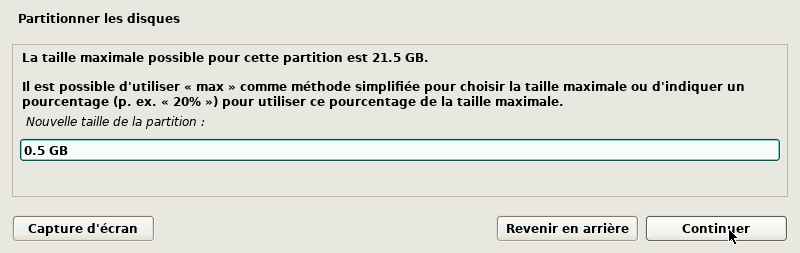
\includegraphics{img049.png}
	\caption{Partition de 0,5 Go}
\end{figure}

La première partition crée est de 512 Mo (en GB : 0,5) qui sera le futur {\tt /boot}, l'installateur refusera d'avoir ce \emph{boot} dans la partition chiffrée, il est donc créé ailleurs.

\begin{figure}
	\centering
	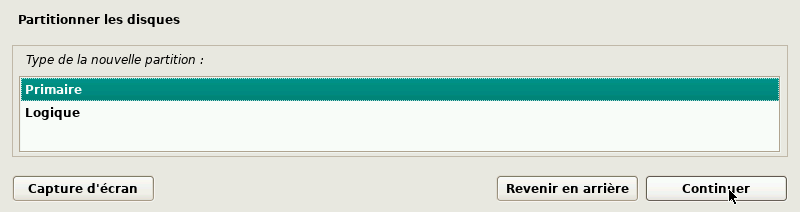
\includegraphics{img050.png}
	\caption{Élémentairement primaire !}
\end{figure}

Comme c'est la première partition créée et qu'elle devra être \emph{bootable} -- démarrable -- alors elle est nécessairement primaire.

Comme le permet le partitionnement BIOS je pourrai installer jusqu'à 4 partitions primaires ou 3 primaires + une vingtaine de secondaires ce qui est la plupart du temps largement suffisant.

Notez que \emph{Windows} (ancien) utilisait à l'époque une seule partition primaire, les autres devant \emph{de facto} être secondaires.

\begin{figure}
	\centering
	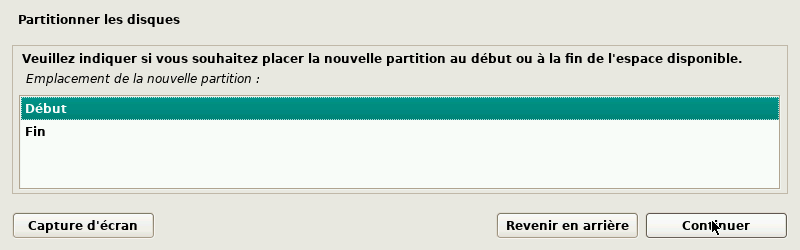
\includegraphics{img051.png}
	\caption{La primaire au début, logique non ?}
\end{figure}

Comme je souhaite que cette partition soit de plus démarrable et que le disque est en DOS, alors il est important que la partition soit placée au début du disque.

\begin{figure}
	\centering
	\includegraphics{img052.png}
	\caption{Pas bootable.}
\end{figure}

La première change à modifier pour cette partition afin de la rendre démarrable est de changer le drapeau ou Indicateur d'armorçage de `` absent'' à `` présent''.

\begin{figure}
	\centering
	\includegraphics{img053.png}
	\caption{Bootable}
\end{figure}

Dans les réglages qui sont aussi modifiés il y a le choix du type de système de fichier dans Utiliser comme, par défaut le type de fichiers journalisé le plus répandu est `` ext4''.

\begin{figure}
	\centering
	\includegraphics{img054.png}
	\caption{Fin du partitionnement de cette partition}
\end{figure}

Une fois les réglages effectués, la partition en question est prête donc on peut en finir avec elle et passer à la suite.

\begin{figure}
	\centering
	\includegraphics{img055.png}
	\caption{Faut-il inscrire les changements ?}
\end{figure}

Cela revient à inscrire dans la table des partitions l'existence de cette nouvelle partition.

\begin{figure}
	\centering
	\includegraphics{img056.png}
	\caption{La racine est créée ! Mais on verra ensuite que c'est une erreur !}
\end{figure}

Ce qui se voit tout de suite dans la fenêtre. 
Attaque du gros morceau qui suit, dans l'espace libre va être créée une nouvelle partition ...

\begin{figure}
	\centering
	\includegraphics{img057.png}
	\caption{création d'une nouvelle partition}
\end{figure}

... qui va occuper tout le reste de l'espace ...

\begin{figure}
	\centering
	\includegraphics{img058.png}
	\caption{qui occupe tout le reste du disque}
\end{figure}

... de type primaire.

\begin{figure}
	\centering
	\includegraphics{img059.png}
	\caption{Primaire !}
\end{figure}

Par défaut cette partition est présentée par le système comme étant de type {\tt ext4} mais évidemment ce qui est recherché est autre par la création d'une partition chiffrée.

\begin{figure}
	\centering
	\includegraphics{img060.png}
	\caption{type : partition chiffrée, non cryptée}
\end{figure}

Du coup l'écran suivant permettra de paramétrer ce chiffrement :

\begin{figure}
	\centering
	\includegraphics{img061.png}
	\caption{partition chiffrée}
\end{figure}

\begin{figure}
	\centering
	\includegraphics{img062.png}
	\caption{activée !}
\end{figure}

l'une des premières choses, vu que le disque est propre, pas besoin de perdre des heures à effacer le contenu du disque avant de créer la partition chiffrée, aussi je passe de oui à non le paramètre \emph{Effacer les données :}

\begin{figure}
	\centering
	\includegraphics{img063.png}
	\caption{Non à l'effacement.}
\end{figure}

De même je garde le chiffrement \emph{AES} même si trois autres sont généralement proposés en plus, et je descend la clé de 256 bits à 128 bits ce qui suffit globalement à protéger le contenu pour un usage un peu sécurisé.

\begin{figure}
	\centering
	\includegraphics{img064.png}
	\caption{128 bits ça suffit ici}
\end{figure}

Ne pensez pas que votre disque résistera à la visite des membres de la police un jour venu si vous êtes vraiment la cible d'opérations de grande envergure, mais, en cas de vol de votre ordinateur, même un très bon informaticien qui n'aurait pas accès à votre mot de passe n'aura pas accès non plus au contenu du disque.

Puis on en a fini avec cette partition ...

\begin{figure}
	\centering
	\includegraphics{img065.png}
	\caption{fin du partitionnement}
\end{figure}

Le retour à l'écran de partitionnement montre la partition 2 de type chiffrée et inactive, ce qui va être rectifié dans l'étape à suivre.

\begin{figure}
	\centering
	\includegraphics{img067.png}
	\caption{On écrit les infos sur le disque ...}
\end{figure}

Après avoir changé le \og~non~\fg{} en \og~oui~\fg{} dans la demande d'écriture des informations sur le disque.

S'en suivra la phase de création des volumes chiffrés.

\begin{figure}
	\centering
	\includegraphics{img068.png}
	\caption{... et on réécrit le disque !}
\end{figure}

\begin{figure}
	\centering
	\includegraphics{img069.png}
	\caption{choix de la partition à chiffrer}
\end{figure}

Il faut bien sûr choisir la partition chiffrée à configurer...

\begin{figure}
	\centering
	\includegraphics{img070.png}
	\caption{et c'est choisi}
\end{figure}

et bien sûr on finit par terminer, ce qui va déclencher l'écran suivant où sera demandé le mot de passe pour déchiffrer la partition créée~:

\begin{figure}
	\centering
	\includegraphics{img071.png}
	\caption{71}
\end{figure}

puis une phase de démarrage des nouveaux outils (en l'occurrence ils s'agit plus que probablement de {\tt dm-crypt} ou {\tt cryptsetup}.

\begin{figure}
	\centering
	\includegraphics{img072.png}
	\caption{progression de l'analyse du disque}
\end{figure}

Cela affichera désormais une nouvelle ligne reprenant le nom de la partition du disque choisi {\tt sda2} devenant {\tt sda2\_crypt} et une nouvelle série de lignes dans le résumé de l'installateur.

\begin{figure}
	\centering
	\includegraphics{img073.png}
	\caption{deux nouvelles lignes !}
\end{figure}

\begin{verbatim}
Volume chiffré (sda2_crypt) - 21.0 GB Linux device-mapper (crypt)
  >   n°1               21.0 GB     f   ext4
\end{verbatim}
et une modification de la ligne plus bas :
\begin{verbatim}
>   n°2  primaire   21.0 GB      K    (sda2_crypt)
\end{verbatim}
Comme par défaut ce système est en {\tt ext4} on va modifier son type immédiatement pour le passer en \emph{logical volume manager} ou \emph{LVM}.

\begin{figure}
	\centering
	\includegraphics{img074.png}
	\caption{passage de l'ext4 ...}
\end{figure}

\begin{figure}
	\centering
	\includegraphics{img075.png}
	\caption{... vers le volume physique LVM}
\end{figure}

et bien évidemment il faut ensuite finir de paramétrer ce \emph{LVM}.

\begin{figure}
	\centering
	\includegraphics{img076.png}
	\caption{fin de la configuration du lvm}
\end{figure}

\begin{figure}
	\centering
	\includegraphics{img077.png}
	\caption{Modification de la ligne sur {\tt sda2\_crypt} et choix suivant.}
\end{figure}

Avec la création de ce {\emph LVM} il y a une modification de la ligne apparue précédemment lors de la création du volume chiffré : 

\begin{verbatim}
Volume chiffré (sda2_crypt) - 21.0 GB Linux device-mapper (crypt)
  >   n°1               21.0 GB     f   lvm
\end{verbatim}

La fin de ligne passe de {\tt ext4} à {\tt lvm} indiquant que la partition chiffrée {\tt sda2\_crypt} est désormais prête à être formatée non comme une partition standard mais comme un volume spécifique appelé gestion logique des volumes.

La capture ci-avant montre aussi quelle ligne sélectionner ensuite dans le but de poursuivre l'installation.

\begin{figure}
	\centering
	\includegraphics{img078.png}
	\caption{Écriture des modifications ext4 -> lvm}
\end{figure}

Évidemment, la première étape consiste à appliquer la modification du partitionnement, à savoir le passage de {\tt ext4} à \emph{LVM} pour la partition {\tt sda2\_crypt} comme le montre la capture précédente.

S'en suit, capture suivante, une première fenêtre indiquant l'état de la configuration du \emph{LVM} : on vient de paramétrer les partitions pour que soit créé un \emph{LVM}, il est donc pour l'instant libre.

\begin{figure}
	\centering
	\includegraphics{img079.png}
	\caption{Premier écran de la gestion du lvm}
\end{figure}

Naturellement, l'installateur propose de créer \emph{ab initio} un groupe de volume comme ligne présélectionnée dans le but de montrer la voie et de faire gagner du temps.

Comme son nom l'indique, un groupe de volume va grouper plusieurs volumes logiques créés au sein du même \emph{LVM}.

\begin{figure}
	\centering
	\includegraphics{img080.png}
	\caption{Je m'appelle totoro.}
\end{figure}

Comme cette installation ne se veut pas pérenne et sert exclusivement d'exemple didactique, je décide d'appeler le groupe de volume par le premier mot venant à mon esprit à ce moment-là : totoro !

Notez qu'il est intéressant de comprendre qu'un \emph{LVM} peut contenir plusieurs disques ou plusieurs partitions venant de un ou plusieurs disques, ce qui est pratique car le \emph{manager} se chargera de gérer la localisation des fichiers au moment de leur écriture ou de leurs modifications.

\begin{figure}
	\centering
	\includegraphics{img081.png}
	\caption{Où se trouve totoro ?}
\end{figure}

Évidemment il faut préciser au \emph{LVM} où se trouvera ce volume logique totoro vu que le \emph{LVM} peut gérer plusieurs disques ou partitions au sein de la même entité.

Dans cette installation, il se trouve \emph{de facto} dans {\tt sda2\_crypt} puisque nous n'avons qu'un seul disque, avec une seule partition servant de support au \emph{LVM}.

\begin{figure}
	\centering
	\includegraphics{img082.png}
	\caption{Sélection du support devant contenir le gestionnaire de volume logique (lvm).}
\end{figure}

\begin{figure}
	\centering
	\includegraphics{img083.png}
	\caption{Retour au menu, légèrement modifié.}
\end{figure}

\paragraph{Une première différence.} Dès lors, le menu résumé s'étoffe~; non seulement la configuration change puisque désormais nous avons `` 1'' à la fin de la ligne \og~Groupe de volumes:~\fg{} indiquant l'existence du groupe de volume.

\paragraph{Autre modification :} La ligne \og~Volumes physiques libres :~\fg{} passe à zéro puisque le volume logique commence à être utilisé, et la ligne \og~Volumes physiques utilisés :~\fg{} passe quant à elle à 1.

Autres modifications dans les choix des actions, plusieurs lignes viennent d'apparaître, celle qui nous intéresse par la suite est celle invitant à \og~créer un volume logique~\fg{}. 

\begin{figure}
	\centering
	\includegraphics{img084.png}
	\caption{Création du volume logique totoro.}
\end{figure}

Comme le \emph{LVM} ne sait pas où créer ce volume logique, il suffit de le lui indiquer :

\begin{figure}
	\centering
	\includegraphics{img085.png}
	\caption{Je vais créer un volume dans totoro (le pauvre).}
\end{figure}

Chaque volume logique doit avoir un nom qui lui est propre, et je vous recommande même qu'il soit unique dans un premier temps.

Ici le premier que je crée sera le swap (on peut créer les volumes dans l'ordre qu'on veut, cela n'a aucune importance.

\begin{figure}
	\centering
	\includegraphics{img087.png}
	\caption{swap}
\end{figure}

Puis je fixe sa taille -- ce qui est un choix délibéré, d'autres options permettent de le rendre plus dynamique, je vous laisse chercher cela par vous-même.

\begin{figure}
	\centering
	\includegraphics{img088.png}
	\caption{swap de 4 Gio = 4096 Mo}
\end{figure}

Puis l'installateur va me refaire revenir au menu de création des volumes logiques, quelques captures prises au passage ...

\begin{figure}
	\centering
	\includegraphics{img086.png}
	\caption{Je crée la racine}
\end{figure}

... et encore d'autres comme le volume \og~racine~\fg{} ou encore celui appelé \og~maison~\fg{} ...

\begin{figure}
	\centering
	\includegraphics{img089.png}
	\caption{Je fixe la taille de la partition racine.}
\end{figure}

On peux fixer la taille par "k", "M" ou encore "G". 

Une fois tous les volumes créés un récapitulatif sera affiche après avoir choisi de finir la configuration du \emph{LVM}.

Attention cependant 8G = 8 milliards d'octets, ce qui est différent de 8Gi = $8 \times 2^{30}$ octets !

Pour ma part, j'ai décidé de mettre 3 partitions dans le \emph{LVM} :
\begin{itemize}
	\item une partition de 8 Go pour la racine
	\item une partition de 4 Gio pour le swap (la ram ne fait que 2 Gio)
	\item une partition du reste pour la maison
\end{itemize}

Pour choisir le reste de l'espace restant il suffit de laisser la quantité affichée au moment de la création du volume.

Si vous voulez savoir où vous en êtes, il suffit de choisir d'afficher les détails de configuration.

\begin{figure}
	\centering
	\includegraphics{img090.png}
	\caption{Récapitulatif avant de commencer le partitionnement.}
\end{figure}

Puis d'aller sur \fbox{{\tt Terminer}} pour que la configuration soit appliquée au disque.

\begin{figure}
	\centering
	\includegraphics{img091.png}
	\caption{Fin de la création des volumes.}
\end{figure}

Toutes ces opérations pourraient se faire en ligne de commande, d'ailleurs en installant une distribution \emph{archlinux} c'est ce qui doit être fait, voilà les commandes que cela donnerait :

\begin{verbatim}
pvcreate /dev/mapper/sda2_crypt
vgcreate totoro /dev/mapper/sda2_crypt
lvcreate totoro -L 4096M -n swap
lvcreate totoro -L 8G -n racine
lvcreate totoro -l +100%FREE -n maison
\end{verbatim}

l'option {\tt -l +100\%FREE} indique au système que la valeur de taille sera relative (l minuscule) et le paramètre indique l'utilisation de la totalité de l'espace libre restant dans le groupe de volume.

l'option {\tt -L} sert à créer une taille fixe définie avec le paramètre qui suivra.

l'option {\tt -n} sert à nommer ce volume.

Dès lors, les volumes sont accessibles de deux façons différentes.
Soit par cette désignation~:
\begin{verbatim}
/dev/totoro/racine
/dev/totoro/swap
/dev/totoro/maison
\end{verbatim}

ou bien celle-ci~:
\begin{verbatim}
/dev/mapper/totoro-racine
/dev/mapper/totoro-swap
/dev/mapper/totoro-maison
\end{verbatim}

On revient ensuite à l'outil de partitionnement.

\begin{figure}
	\centering
	\includegraphics{img092.png}
	\caption{Redémarrage du partitionnement.}
\end{figure}

Plein de nouvelles lignes arrivent désormais, j'ai volontairement centré la fenêtre sur ces nouvelles lignes, ce qui a caché les autres placées plus bas dans la fenêtre mais accessibles grâce à l'ascenseur à droite de la fenêtre.

\begin{figure}
	\centering
	\includegraphics{img093.png}
	\caption{De nouvelles lignes sont apparues !}
\end{figure}

Il est donc nécessaire de repasser sur chacune de ces nouvelles lignes qui ne sont en rien configurées pour l'heure afin de leur attribuer un formatage et un point de montage dans le système futur.

Il faudra donc passer par les différentes étapes -- je ne commente pas pour l'instant dans cette première version les quelques captures suivantes, les commentaires des images étant explicites.

D'abord je décide de configurer le \emph{swap}.

\begin{figure}
	\centering
	\includegraphics{img094.png}
	\caption{On change ce paramètre car la partition va être utilisée.}
\end{figure}

\begin{figure}
	\centering
	\includegraphics{img095.png}
	\caption{Le type de ce volume sera du swap}
\end{figure}

\begin{figure}
	\centering
	\includegraphics{img096.png}
	\caption{La configuration du swap est finie.}
\end{figure}

\begin{figure}
	\centering
	\includegraphics{img097.png}
	\caption{Le swap est configuré, la ligne correspondante est modifiée, next !}
\end{figure}

Maintenant ça sera le tour de la racine, \emph{root} en anglais, symbolisé par le point de montage {\tt /} dans un système \emph{UNIX} ou \emph{Linux}.

\begin{figure}
	\centering
	\includegraphics{img098.png}
	\caption{La racine sera formatée au type ext4.}
\end{figure}

Puis il faut lui préciser le \og~point de montage~\fg{} ...

\begin{figure}
	\centering
	\includegraphics{img099.png}
	\caption{Le volume racine sera monté dans {\tt /} (la racine!)}
\end{figure}

C'est fini pour la racine. Prochaine étape, le volume où seront les données des utilisateurs c'est-à-dire \texttt{/home} d'où le choix du nom de volume \og~maison~\fg{} pour le désigner.

\begin{figure}
	\centering
	\includegraphics{img100.png}
	\caption{Choix du volume qui va accueillir le \emph{/home}}
\end{figure}

Je vous zappe un des écrans, on passe directement aux réglages :

\begin{figure}
	\centering
	\includegraphics{img101.png}
	\caption{{\tt /home} est configuré au format {\tt ext4}.}
\end{figure}

Retour à l'écran de formatage, cette fois-ci la capture est centrée afin de faire apparaître toutes les partitions.

\begin{figure}
	\centering
	\includegraphics{img102.png}
	\caption{Tout est prêt pour être formaté !}
\end{figure}

Comme vous le voyez, une multitude de lignes sont apparues depuis le début de la configuration, mais, allez-vous être plus attentif ou attentive que je ne l'ai été lors de cette installation, en effet ai-je commis une erreur ?

Oui ? Non ? Je clique sur la dernière ligne pour terminer la phase d'installation ...

\begin{figure}
	\centering
	\includegraphics{img103.png}
	\caption{On y va !}
\end{figure}

... ah ben ... il y avait un problème !

\begin{figure}
	\centering
	\includegraphics{img104.png}
	\caption{boulette !}
\end{figure}

Oups j'ai fait une boulette ! La précipitation lors de la première phase d'installation fait que la première partition {\tt /dev/sda1} qui aurait naturellement dû être associée au point de montage {\tt /boot} a été automatiquement associée à la racine {\tt /}et par manque de vigilance je n'ai pas noté cela.

L'installateur a repéré mon erreur. Il me le signale par le message de cette boite de dialogue.

\begin{figure}
	\centering
	\includegraphics{img105.png}
	\caption{Correction du point de montage de {\tt /dev/sda1}}
\end{figure}

Je modifie donc le point de montage de {\tt /dev/sda1} pour qu'il soit bien sur {\tt /boot} et non sur {\tt /} comme tout à l'heure...

\begin{figure}
	\centering
	\includegraphics{img106.png}
	\caption{Erreur corrigée !}
\end{figure}

... et c'est parti !

\begin{figure}
	\centering
	\includegraphics{img107.png}
	\caption{Terminer le partitionnement et appliquer les changements}
\end{figure}

La configuration des différents lecteurs, la correction du bug introduit et surtout le montage et les choix opérés sur le disque sont désormais finis, il est temps de passer à l'étape suivante.

\begin{figure}
	\centering
	\includegraphics{img108.png}
	\caption{Fenêtre de confirmation totale de tous les réglages}
\end{figure}

Avant de procéder aux modifications, il est demandé de vérifier dans cette fenêtre que les choix saisis, les partitions créées et tous les volumes spécifiques sont prêts, par défaut le choix est non évidemment, ce qui évite qu'en cas d'appui malencontreux la procédure continue...

\begin{figure}
	\centering
	\includegraphics{img109.png}
	\caption{Fenêtre de confirmation totale de tous les réglages : OUI !}
\end{figure}

... mais étant sûr du choix, c'est l'heure de procéder !

\begin{figure}
	\centering
	\includegraphics{img110.png}
	\caption{Barre progression création partitions}
\end{figure}

Le disque est prêt. 
Il faut désormais installer le squelette du futur système avec le \og~sytème de base~\fg{}.

\chapter{Installation du système de base sur la cible}

Puisque le disque est partitionné et formaté comme souhaité il est désormais temps de passer à l'installation du squelette du futur système opératif. 
Ce squelette est désigné par le \og~système de base~\fg{} dans l'installateur.

\begin{figure}
	\centering
	\includegraphics{img111.png}
	\caption{111}
\end{figure}

Pas grand chose à faire hormis exécuter l'étape d'installation puisque cette structure est parfaitement automatisée et installe les outils nécessaires à l'administration ou aux réparations d'un Linux en place. 
L'utilisateur moyen ou son pendant féminin ne saura peut-être jamais que ces programmes existent.

\begin{figure}
	\centering
	\includegraphics{img112.png}
	\caption{112}
\end{figure}

Une question est posée cependant : quel noyau choisir dans ce système basique ? On pourrait avoir l'idée de dire aucun (mais je n'ai jamais testé), choisir un {\tt linux-image-numéros-architecture} figera le noyau dans cette version malgré les mises à jour, par contre l'utilisation de la ligne {\tt linux-image-architecture} comme sur la capture où on voit le fichier pour l'architecture {\tt amd64} désignant les processeurs 64 bits (\emph{Intel, AMD} ...) habituels sur PC.

\begin{figure}
	\centering
	\includegraphics{img113.png}
	\caption{113}
\end{figure}

Enfin il est posé la question concernant la liste des pilotes du noyau à installer. Dans le monde \emph{Windows}` ces pilotes sont 
appelés \emph{drivers} et permettent de reconnaître du matériel. 
Sur un appareil fixe qui ne recevra aucun matériel supplémentaire on peut choisir la ligne \emph{image ciblée}, mais pour un ordinateur qui pourra recevoir des disques, des imprimantes, des scanners ou d'autres périphériques il est préférable de choisir \emph{image générique} qui installera la totalité des pilotes du noyau disponibles.

\begin{figure}
	\centering
	\includegraphics{img114.png}
	\caption{114}
\end{figure}

Le système de base étant prêt, désormais il va falloir configurer l'outil en charge d'installer des logiciels supplémentaire connu sous le nom de \og~gestionnaire de paquets~\fg{}.

\chapter{Configuration de l'outil de gestion des paquets}

L'outil de gestion des paquets est le programme utilisant une des méthodes d'installation des programmes. Linux en connaît quatre qui peuvent plus ou moins rangés en trois modes :
\begin{itemize}
	\item installation d'un paquet~:
	\begin{itemize}
		\item par le gestionnaire des paquets (graphique / textuel)
		\item manuellement (graphique / textuel)
		\item via un \emph{Store} comme sur téléphone mobile (graphique)
	\end{itemize}
	\item exécution d'un binaire prêt-à-l'emploi (graphique / textuel)
	\item compilation des sources et installation manuellement (textuel)
\end{itemize}

Au moment de l'installation, \emph{Debian} va proposer de configurer l'outil de gestion des paquets (il n'y a pas de \emph{Store} dans le style d'un \emph{Apple/Windows/Ubuntu store}) propre à cette distribution et qui se trouve également dans ses distributions filles.

\begin{figure}
	\centering
	\includegraphics{img115.png}
	\caption{Menu principal, ligne de la configuration du  gestionnaire de paquets}
\end{figure}

Dans un premier temps il faut préciser si d'autres supports d'installation sont fournis. Par défaut avec l'image téléchargée ce n'est pas le cas, aussi la réponse "non" est présélectionnée et suffit amplement.

\begin{figure}
	\centering
	\includegraphics{img116.png}
	\caption{Analyse d'un nouveau support}
\end{figure}

Je profite cependant pour rappeler que si j'ai choisi cette distribution ça n'est pas le fruit du hasard. 
\emph{Debian} fait partie des rares distributions entièrement disponible \emph{off line} et à ce titre en cas de chute mondiale du réseau internet pendant une durée assez longue pour avoir besoin de réinstaller un système opératif, alors il est possible d'avoir besoin des DVD de la distribution complète.

Dans ce cas, \emph{Debian} offre 4 DVD contenant la plus grande partie des logiciels disponibles et arrivé(e) à cette étape de l'installation il suffira de cocher \fbox{oui} et de suivre les étapes qui s'afficheront (principalement insérer les nouveaux DVD dans le lecteur, valider pour que le système les parcoure puis à la fin de la lecture de tous les DVD, remettre le premier pour poursuivre l'installation.

\begin{figure}
	\centering
	\includegraphics{img117.png}
	\caption{Mise en place d'un dépôt en réseau ?}
\end{figure}

C'est alors que l'installateur va demander le type de connexion à établir avec le serveur de paquet, par défaut il s'agit d'une connexion {\tt http} ce qui suffit sachant que les signatures des paquets sont déjà récupérées ailleurs, la comparaison des \emph{hashes} entre le paquet téléchargé et la signature attendue permettra de savoir si le paquet est corrompu ou non.

\begin{figure}
	\centering
	\includegraphics{img118.png}
	\caption{Choix du type de connexion au serveur de paquets}
\end{figure}

Notez que l'autre choix, {\tt https}, nécessitera l'installation du paquet {\tt apt-https-transport} quant à celui en {\tt ftp} j'avoue ne jamais l'avoir utilisé.

\begin{figure}
	\centering
	\includegraphics{img119.png}
	\caption{Choix de la région de localisation du dépôt.}
\end{figure}

Une fois le type de connexion au dépôt choisi, il est bien temps de configurer la région du monde où sélectionner le serveur qui stocke déjà les paquets, évidemment étant en France, je choisis le dépôt français, espérant ainsi limiter l'impact de la connexion.

Ce choix est déjà effectué par défaut d'ailleurs, se basant sur la localisation linguistique déclarée auparavant.

\begin{figure}
	\centering
	\includegraphics{img120.png}
	\caption{Choix précis du serveur}
\end{figure}

Ensuite vient la sélection plus précise du serveur, l'image ci-avant montre le choix par défaut que je ne change pas.

\begin{figure}
	\centering
	\includegraphics{img121.png}
	\caption{Configuration du proxy}
\end{figure}

Dans certains cas, typiquement dans un réseau d'entreprise ou dans un réseau administratif, les connexions à internet sont soumises à identification et authentification de l'utilisateur, il s'agit alors de configurer le proxy correspondant.

Le proxy étant le serveur qui gère le transit des pages internet par le protocole {\tt http} et/ ou {\tt https} voire aussi les autres. 
Maintenant passons au choix des familles paquets.

Ceci reviendra à configurer le fichier {\tt /etc/apt/sources.list}.

\begin{figure}
	\centering
	\includegraphics{img122.png}
	\caption{Activation des paquets non-libres.}
\end{figure}

Toujours dans la configuration de l'outil de gestion des paquets, il est temps de savoir si vous ne voulez faire apparaître que les paquets libres -- par défaut \emph{Debian} ne propose que les paquets libres -- ou bien si vous désirez accéder à des paquets non-libres.

Typiquement le fichier qui va être écrit est {\tt /etc/apt/source.list} ou bien, dans les debian plus modernes, une série de fichiers situés dans le dossier {\tt /etc/apt/sources.list.d}.

Plusieurs configurations sont alors possibles, et, vu le choix de la capture d'écran précédente, une image n'apparaîtra pas, aussi vais-je vous expliquer les différence.

\paragraph{Si on répond non à l'utilisation des logiciels non-libres} alors une nouvelle fenêtre va s'ouvrir demandant si on souhaite utiliser des logiciels avec des bibliothèques non-libres.

\paragraph{si on répond également non à l'utilisation de logiciels libres utilisant des bibliothèques non-libres} dans ce cas l'installation passera à la configuration des sources dans le fichier de gestion des paquets.

\paragraph{Si on répond oui à l'utilisation des logiciels non-libres} alors la question suivante passera directement au choix faisant apparaître les sources dans le fichier de configuration des paquets.

\begin{figure}
	\centering
	\includegraphics{img123.png}
	\caption{Activation des sources ?}
\end{figure}

Ici les sources sont par défaut proposées actives, mais, comme je ne pense pas développer des programmes depuis Linux nécessitant les sources des paquets, alors je répond bien évidemment non.

\begin{figure}
	\centering
	\includegraphics{img124.png}
	\caption{Je n'en ai pas besoin !}
\end{figure}

Et pendant que les téléchargements de fichiers vont continuer, je prends le temps d'expliquer les différences.

\begin{figure}
	\centering
	\includegraphics{img125.png}
	\caption{téléchargement des fichiers contenant la liste des paquets et de leurs versions}
\end{figure}

Je vais supposer l'hypothèse d'un fichier unique sis en {\tt /etc/apt} qui sera juste le {\tt source.list} unique. La distribution \emph{debian} correspondante étant \emph{bullseye} à savoir la version 11.2 actuellement stable.

Voici la version si seuls les paquets libres et les sources sont actives~:

\begin{verbatim}
deb http://deb.debian.org/debian bullseye main
deb-src http://deb.debian.org/debian bullseye main

deb http://deb.debian.org/debian-security/ bullseye-security main
deb-src http://deb.debian.org/debian-security/ bullseye-security main

deb http://deb.debian.org/debian bullseye-updates main
deb-src http://deb.debian.org/debian bullseye-updates main
\end{verbatim}

Voici la version si seuls les paquets libres sont actifs et les sources sont désactivées~:

\begin{verbatim}
deb http://deb.debian.org/debian bullseye main
\chapter{deb-src http://deb.debian.org/debian bullseye main

deb http://deb.debian.org/debian-security/ bullseye-security main
\chapter{deb-src http://deb.debian.org/debian-security/ bullseye-security main

deb http://deb.debian.org/debian bullseye-updates main
\chapter{deb-src http://deb.debian.org/debian bullseye-updates main
\end{verbatim}

Voici la version du fichier avec les paquets libres activés mais aucune source activée~:

\begin{verbatim}
deb http://deb.debian.org/debian bullseye main

deb http://deb.debian.org/debian-security/ bullseye-security main

deb http://deb.debian.org/debian bullseye-updates main
\end{verbatim}

Voici la version du fichier sans sources, avec paquets libres et aussi bibliothèques non-libres (contrib)~:

\begin{verbatim}
deb http://deb.debian.org/debian bullseye main contrib

deb http://deb.debian.org/debian-security/ bullseye-security main contrib

deb http://deb.debian.org/debian bullseye-updates main contrib
\end{verbatim}
et enfin voici la version du fichier sans sources, avec paquets libres, non-libres et donc par défaut les bibliothèques non-libres incluses~:

\begin{verbatim}
deb http://deb.debian.org/debian bullseye main contrib non-free

deb http://deb.debian.org/debian-security/ bullseye-security main contrib non-free

deb http://deb.debian.org/debian bullseye-updates main contrib non-free
\end{verbatim}

\begin{figure}
	\centering
	\includegraphics{img126.png}
	\caption{Activation des \emph{backports}}
\end{figure}

L'étape suivante -- celle de la capture -- demande si l'utilisateur désire activer les \emph{backports}, c'est-à-dire les logiciels rétro-portés de la future version -- en l'occurrence \emph{debian 12 bookworm} -- mais qui sont transposables car compatibles en l'état avec la version actuelle.

À titre personnel j'aime beaucoup avoir les \emph{backports} activés car cela donne au système une grande stabilité tout en ayant des versions logicielles assez récentes, surtout au bout de 2 ou 3 ans de version stable.

\begin{figure}
	\centering
	\includegraphics{img127.png}
	\caption{Récupération des backports si activé}
\end{figure}

Dans le cas de l'activation de ce dépôt spécifique, une série de fichiers sera téléchargés.

\paragraph{Notez que} pour installer un logiciel depuis ce dépôt on peut soit éditer le fichier {\tt /etc/apt/apt.conf} ou l'un des fichiers dans le fichier {\tt /etc/apt/apt.conf.d/99debian-backports} (au besoin le créer) puis ajouter~:

\begin{verbatim}
Package: *
Pin: release a=stretch-backports
Pin-Priority: 900
\end{verbatim}
source : \url{https://wiki.debian.org/AptConfiguration}

Plus la priorité est élevée, plus ce dépôt sera préféré.

Si on désire ne pas toucher au système de façon permanente, il est possible de procéder à une mise à jour en forçant le choix du dépôt par l'ajout de l'option {\tt -t debian-backports} par exemple lors d'une installation ou d'une mise à jour~:

\begin{verbatim}
apt update
apt -t bullseye-backports upgrade
\end{verbatim}

forcera l'installation des paquets depuis {\tt bullseye-backports} si ce dépôt est évidemment présent dans {\tt /etc/apt/sources.list} ou dans un fichier présent dans {\tt /etc/apt/sources.list.d/}.

\chapter{Installation des logiciels initiaux}

Au moment de l'installation est proposé de directement mettre sur le disque final une série de logiciels prêts à l'emploi afin de permettre à l'utilisateur d'avoir un environnement opérationnel et pré-paramétré par défaut.

Bien que beaucoup d'utilisateurs de \emph{Debian} l'utilisent en mode serveur, l'installateur propose dès le début les plus classiques environnements graphiques et des outils divers tels que les outils bureautiques ou des navigateurs internet par défaut et installables par une simple coche de case.

\begin{figure}
	\centering
	\includegraphics{img128.png}
	\caption{}
\end{figure}

C'est ce qui est proposé dans la ligne \emph{Choisir et installer des logiciels}.

Une fois ce choix enclenché une phase de mise à jour -- d'où la nécessité de la connexion active -- commence afin de proposer l'installation immédiate de leurs dernières versions disponibles.

\begin{figure}
	\centering
	\includegraphics{img129.png}
	\caption{}
\end{figure}

L'installateur propose aussi d'aller rechercher les mises à jour de sécurité des logiciels soit déjà installés par l'étape de création du système de base, soit des logiciels qui sont installés à cette étape-ci.

\begin{figure}
	\centering
	\includegraphics{img130.png}
	\caption{}
\end{figure}

Une phase temporaire de téléchargements s'opère...

\begin{figure}
	\centering
	\includegraphics{img131.png}
	\caption{}
\end{figure}

... suite à quoi il est demandé si l'on souhaite -- ou non -- participer aux remontées d'expérience et de \emph{bugs} pour aider les 
programmeurs ou mainteneurs du projet dans l'amélioration des paquets logiciels concernés.

\begin{figure}
	\centering
	\includegraphics{img132.png}
	\caption{}
\end{figure}

Après plusieurs téléchargements et mises à jour récupérées l'utilitaire {\tt tasksel} est téléchargé ... puis commence à s'exécuter.

\begin{figure}
	\centering
	\includegraphics{img133.png}
	\caption{}
\end{figure}

Cet outil, {\tt tasksel}\footnote{\emph{
tasksel} pour \emph{tasks select} il s'agit de choisir une ou plusieurs grandes lignes directrices attribuées au système, installant ainsi des outils en lien avec les tâches à accomplir, profilant par la même la machine.} propose alors de cocher des \textbf{meta-paquets} qui sont des paquets de paquets, ou groupes de paquets si cela est plus clair, et dont le but est d'installer des environnements prêts à utiliser avec tout ce qu'il faut pour apprécier un système fonctionnel.

\begin{figure}
	\centering
	\includegraphics{img134.png}
	\caption{}
\end{figure}

Une fois les cases cochées et la touche Continuer enfoncée c'est le moment où l'installation du système initial et de tous les paquets se fera sans qu'on ai besoin de quoi que ce soit.

\begin{figure}
	\centering
	\includegraphics{img135.png}
	\caption{}
\end{figure}

Cette étape est la partie la plus longue de toute l'installation puisque dépendant de la quantité de paquets à télécharger suivant les cases du menu précédent choisies mais également du débit de la connexion internet utilisée pour récupérer l'intégralité de ces paquets.

Cette dépendance est principalement effective sur la première partie du processus : celle du téléchargement des logiciels.

Allez faire une promenade, ou préparer un gâteau ça peut être long.

Ne vous fiez pas à la barre de progression : la quantité totale des téléchargements correspond à 1/3 de la barre, le second tiers est l'installation des paquets suite à leur décompression et le dernier tiers est dédié au paramétrage initial de chaque paquet.

Une fois tous les paquets récupérés, ce qui fera la rapidité ou à contrario la lenteur de la progression seront les performances intrinsèques de la machine.

\chapter{L'installation du chargeur de démarrage}

C'est à ce moment de l'installation que la coupure de courant a eu lieu par manque d'anticipation de ma part et un chargeur non branché à temps.

Aussi les captures suivantes sont issues de la 2e installation qui a suivi. 
Je n'ai pas opté cette fois-ci par habitude et réflexe à une installation en mode graphique experte mais en mode experte textuelle aussi pardonnerez-vous la différence de présentation des contenus des captures bien que les messages affichés soient les mêmes que ceux de l'installation experte graphique.

\begin{figure}
	\centering
	\includegraphics{img136.png}
	\caption{}
\end{figure}

Par défaut depuis longtemps l'installateur est \emph{GRUB}. Il prend en charge le démarrage et le lancement de de l'image de démarrage.

L'un des premiers travaux est de rechercher dans l'ordinateur les autres systèmes d'exploitation, tâche confiée à l'outil appelé 'os prober'.

Comme l'installation s'est faite depuis un disque vierge sans autre système d'exploitation présent, la détection renvoie un résultat nul et le message suivant apparaît.

\begin{figure}
	\centering
	\includegraphics{img137.png}
	\caption{}
\end{figure}

Une fois le message passé, ce nouveau message sera affiché, il demande à l'utilisateur d'indiquer un disque sur lequel sera installé la première partie de grub dans le \emph{MBR}\footnote{MBR = \emph{Master Boot Record}. 
C'est la zone du disque placée à son début qui est utilisée pour indiquer au système où se trouve le système d'exploitation. 
Ceci est caractéristique des systèmes \emph{BIOS}. 
Un autre système existe dans les machines en \emph{EFI}.} du disque. 
Si plusieurs disques sont présents il faut faire attention à ne pas se tromper.

\begin{figure}
	\centering
	\includegraphics{img138.png}
	\caption{}
\end{figure}

Vient le moment de l'installation dédié à l'\emph{EFI}. 
Cette installation ayant été menée dans un système non-\emph{EFI} forcément ... pas besoin d'obliger le système à forcer le déroutement du chemin naturel de l'installation du mode \emph{EFI}.

\begin{figure}
	\centering
	\includegraphics{img139.png}
	\caption{}
\end{figure}

%<!-- \includegraphics{img140.png} image inutile car en double -->

L'installation de \emph{GRUB} s'effectue alors dans le premier disque ({\tt sda}) ce qui peut demander un petit moment.

\begin{figure}
	\centering
	\includegraphics{img141.png}
	\caption{}
\end{figure}

Puis automatiquement le script de création et/ou mise-à-jour de la configuration de \emph{GRUB}.

\begin{figure}
	\centering
	\includegraphics{img142.png}
	\caption{}
\end{figure}

Ces deux phases sont totalement automatiques et une fois fini c'est la fin de l'installation qui s'annonce.

À ce stade la machine devient démarrable puisque \emph{GRUB} est installé mais le noyau installé n'est pas optimisé pour l'ordinateur, cette adaptation sera faite lors de la phase finale qui suit.

\chapter{La phase finale de l'installation}

On arrive à la fin du spectacle. Il ne reste plus qu'à paramétrer les utilisateurs et recréer une image propre pour le démarrage.

Le grand menu d'accueil nous indique d'ailleurs qu'on arrive à \og~Terminer l'installation~\fg{} c'est tout dire. 
Et on valide !

\begin{figure}
	\centering
	\includegraphics{img143.png}
	\caption{}
\end{figure}

Tous les paramètres saisis tout à l'heure sont mis en place maintenant : création des utilisateurs avec inscription de l'utilisateur standard dans le groupe \og~sudo~\fg{} si le compte {\tt root} n'est pas activé.

\begin{figure}
	\centering
	\includegraphics{img144.png}
	\caption{}
\end{figure}

Vient ensuite l'exécution du script {\tt hw-detect} dont le nom est suffisamment clair pour supposer qu'il est là pour détecter le matériel spécifiquement. 
Je pense qu'il sert dans l'étape de compilation de l'initramfs à venir plus loin.

\begin{figure}
	\centering
	\includegraphics{img145.png}
	\caption{}
\end{figure}

Puis une fois ceci effectué l'installateur demande si l'horloge matérielle est déjà en UTC (par exemple si l'ordinateur utilisait déjà un système Linux ou UNIX) ou pas afin de correctement synchroniser l'heure système et l'heure matérielle.

\begin{figure}
	\centering
	\includegraphics{img146.png}
	\caption{}
\end{figure}

Avant que le système soit pleinement opérationnel il reste une phase automatique qui est la génération de l'image initiale au démarrage. 
Il faut comprendre qu'un système Linux est très particulier sur sa phase de démarrage : en effet un micro-système non-interactif est exécuté au tout début, ce système ayant pour charge de vérifier l'intégrité du système à venir, il est de très petite taille mais doit contenir l'essentiel pour accomplir sa tâche.

Ce système est appelé \emph{initramfs}\footnote{initramfs : Système de Fichiers Initial chargé en mémoire RAM. Son rôle est de charger un système quasiment non-interactif dont le but est de vérifier que le système Linux est opérationnel et en état, ses seules interactions consistent en l'accès donné pour du dépannage restreint.} ou encore {\tt initcpio} et il est généré dans les distributions de type \emph{Debian} par la commande :

\begin{verbatim}
update-initramfs -k all -u
\end{verbatim}

Si les options diffèrent un peu -- et sûrement -- lors de l'installation, c'est quand même cet outil qui es exécuté à ce moment de l'installateur.

C'est dans cette étape que sont à mon avis utilisées les informations récupérées par le script {\tt hw-detect} aux étapes précédentes.

\begin{figure}
	\centering
	\includegraphics{img147.png}
	\caption{}
\end{figure}

Pour finir enfin, la dernière étape vous signaler la démarche à suivre dans ce dernier message.

\begin{figure}
	\centering
	\includegraphics{img148.png}
	\caption{}
\end{figure}

Voilà ! Vous êtes prêt(e) à utiliser ce système fraîchement installé et qui je l'espère vous ouvrira de nouvelles aventures dans le monde du libre et de Linux.

Amusez-vous bien !

\chapter{Le démarrage qui suit}

Les pages qui suivent vont montrer quelques captures d'écran du résultat obtenu. 
Comme l'installation est relativement minimaliste aussi GRUB est-il en version textuelle et non graphique. 
Il reste évidemment paramétrable en allant chercher les fichiers idoine.

L'écran devrait ressembler à celui qui suit (j'ai inversé les couleurs de la zone autour du rectangle bleu central)

\begin{figure}
	\centering
	\includegraphics{img149.png}
	\caption{}
\end{figure}

Très rapidement après la disparition de l'écran précédent et vu que le disque dur est chiffré, le mot de passe est à saisir (la capture d'écran est en couleurs inversées pour économiser l'encre). 
Il y a par défaut 3 tentatives autorisées avant que le système ralentisse l'accès.

\begin{figure}
	\centering
	\includegraphics{img150.png}
	\caption{}
\end{figure}

Plusieurs lignes apparaîtront avec le démarrage de plusieurs services, tant que des OK, ou de INFO apparaissent tout va bien, attention dans le cas des WARN (orange) et surtout s'il y a des FAILED (rouge) visibles il faudra agir.

La capture d'écran suivante est en couleurs inversées aussi.

\begin{figure}
	\centering
	\includegraphics{img151.png}
	\caption{}
\end{figure}

Arrivera alors l'écran d'identification et d'authentification le plus simple possible.

\begin{figure}
	\centering
	\includegraphics{img152.png}
	\caption{}
\end{figure}

Voici le bureau obtenu ensuite avec l'explorateur de fichiers à gauche et un terminal à droite.

\begin{figure}
	\centering
	\includegraphics{img153.png}
	\caption{}
\end{figure}

Le bureau vide de LXDE sur debian 11.2~:
\begin{figure}
	\centering
	\includegraphics{img154.png}
	\caption{}
\end{figure}

Pour finir : les messages d'extinction en couleurs inversées afin d'économiser aussi l'encre..
\begin{figure}
	\centering
	\includegraphics{img155.png}
	\caption{}
\end{figure}

\chapter{Remerciements et mentions.}

Avant de finir ce document je souhaite ici remercier les quelques personnes qui ont participé à la finalisation de ce document soit par leurs relectures et corrections apportées, soit par les conseils qu'elles ont pu me prodiguer afin d'améliorer la lisibilité et la clarté de ce discours.

Je remercie donc Olivier \bsc{Jeulin} et Florence \bsc{Gain} pour leurs conseils et leur patience à la lecture ou la relecture du document, je remercie doublement Olivier d'ailleurs pour tout le temps, la technicité et la gentillesse dont il a fait preuve également pour la création de la couverture et de la 4\ieme{}.

Toute cette installation a été réalisée avec l'outil {\tt virtualbox} présent dans la distribution Linux \emph{Ubuntu} 22.04 en pré-version car elle ne sortira que dans deux mois officiellement. 
Vous me direz que c'est paradoxal d'utiliser une autre distribution et je vous dirai que cela l'est mais que cet ordinateur utilisé avec Ubuntu est dédié à un membre de ma famille qui va justement débuter sous Linux et que ce fût aussi l'occasion pour moi de réutiliser cette distribution que j'avais oublié depuis longtemps.

\paragraph*{Mon avis sur Ubuntu ?} 
Je vous le partagerai ultérieurement car lorsque j'ai divergé de son utilisation en 2010 c'était pour des raisons qui sont encore d'actualité -- donc vous avez mon avis -- et son évolution bien qu'honorable ne correspond pas ou plus à mes besoins.

Les captures d'écran ont été réalisées avec l'outil intégré à {\tt virtualbox} et retouchées ensuite une à une avec {\tt kolourpaint} car pour réduire les espaces de façon différente pour chaque image il ne pouvait être question de faire un traitement par lot.

La saisie du code source du document en langage {\tt Markdown} a été effectuée dans le bloc-notes {\tt mousepad} dans l'environnement graphique \emph{XFce4}. 
L'exportation dans des formats autres (html, pdf) provient de l'emploi de l'utilitaire {\tt pandoc} en version 2.9.2.1.

\newpage
\renewcommand{\baselinestretch}{1}
\setlength{\parskip}{0em}
\listoffigures

\newpage
\pagenumbering{gobble}
~
\vfill
\begin{figure}
	\centering
	\begin{tikzpicture}
		\draw[dashed] (0,0) rectangle (0.95\linewidth,23) ;
	\end{tikzpicture}
\end{figure}
\vfill
~

\end{document}